%!TEX root = ../thesis.tex
% ******************************* Thesis Appendix B ********************************

\chapter{Supplementary Figures}
\clearpage

%\section{Additional results for Chapter 2}

% \begin{figure}[H]
%     \centering
%     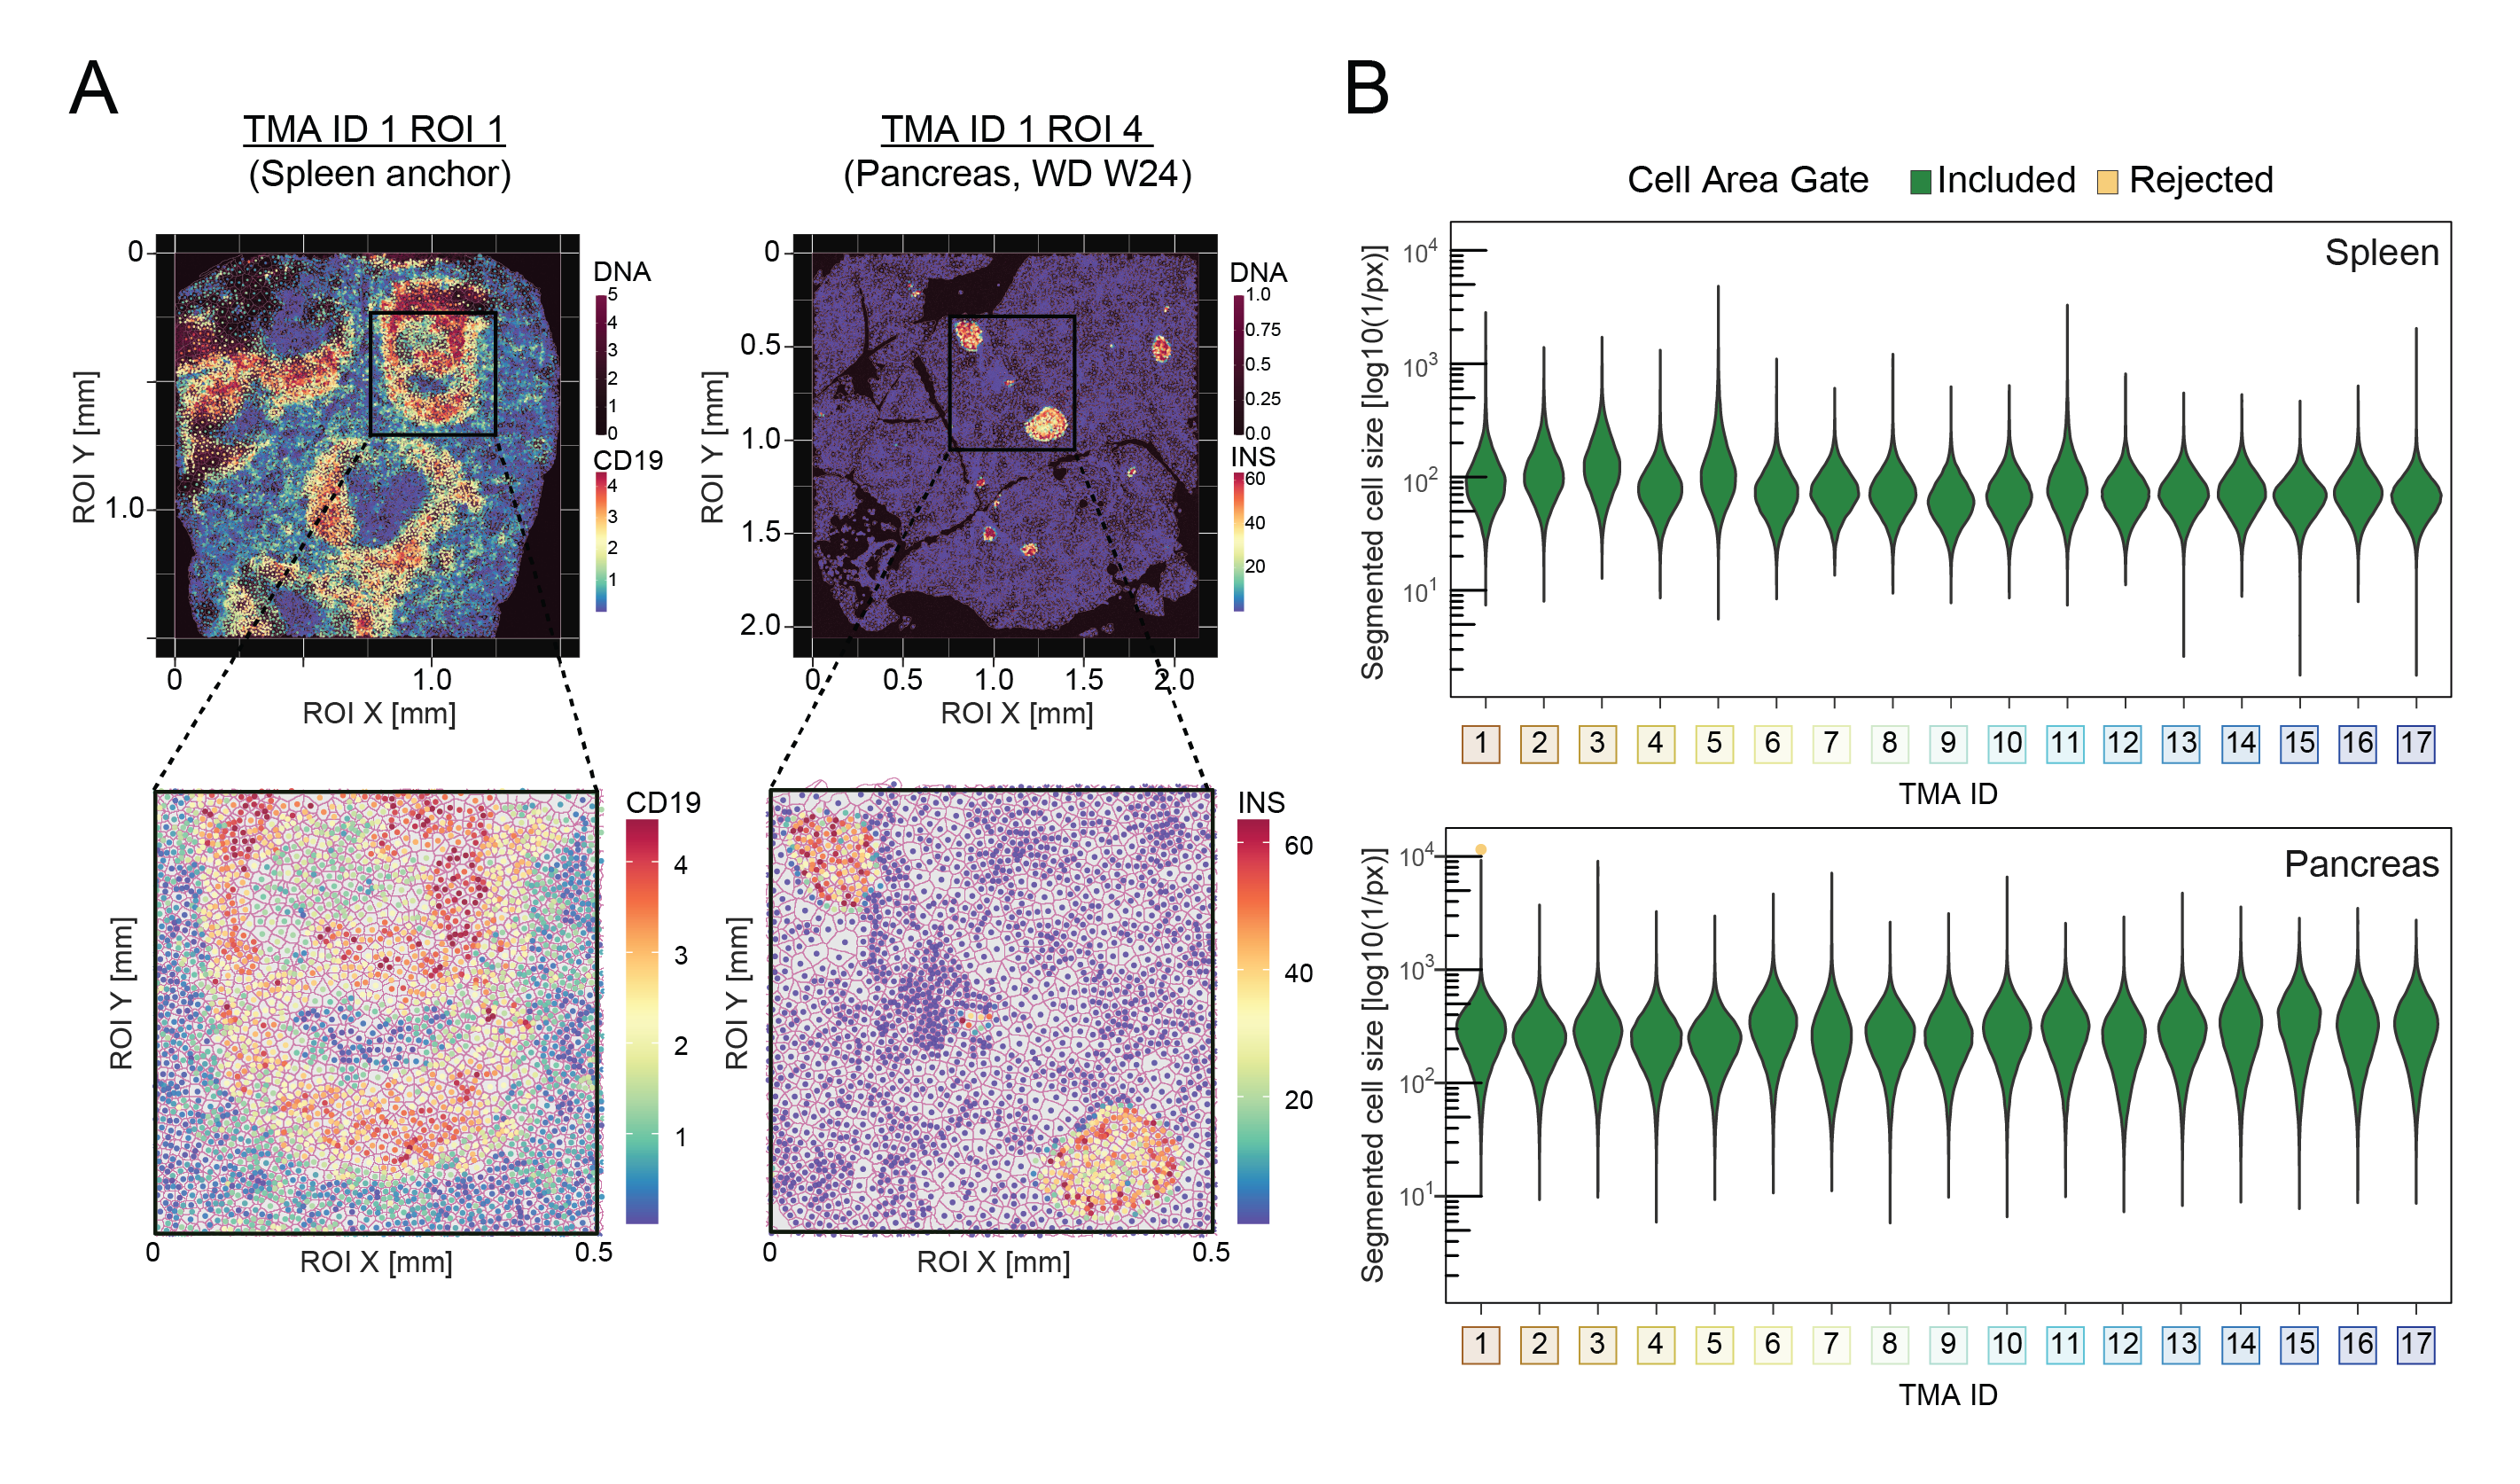
\includegraphics[width=\linewidth]{Appendix2/Fig/F2-A4-01.png}
%     \caption[IMC Segmentation Workflow]{\textbf{IMC Segmentation Workflow}\\
%     \textbf{(A)} Representative segmentation masks of ablated ROIs in anchor spleen (left) and pancreas (right) sections, zoomed in to 500 µm on each ROI for better visibility. For better orientation, average expression of CD19 (left) and INS (right) of each segmented cell are additionally drawn as dots. Dimensions of each ROI are denoted on both axes (1 pixel per µm resolution). \textbf{(B)} Violin plots depicting the log10-transformed pixel count (indicating cell size) within each segmented cell across all TMAs from all analyzed samples. Cells larger than 10000 px, potentially representing doublets, were highlighted in yellow and removed from downstream analysis.}
%     \label{suppl_fig:imc_segmentation}
% \end{figure}

% % \begin{figure}[htbp]
% %     \centering
% %     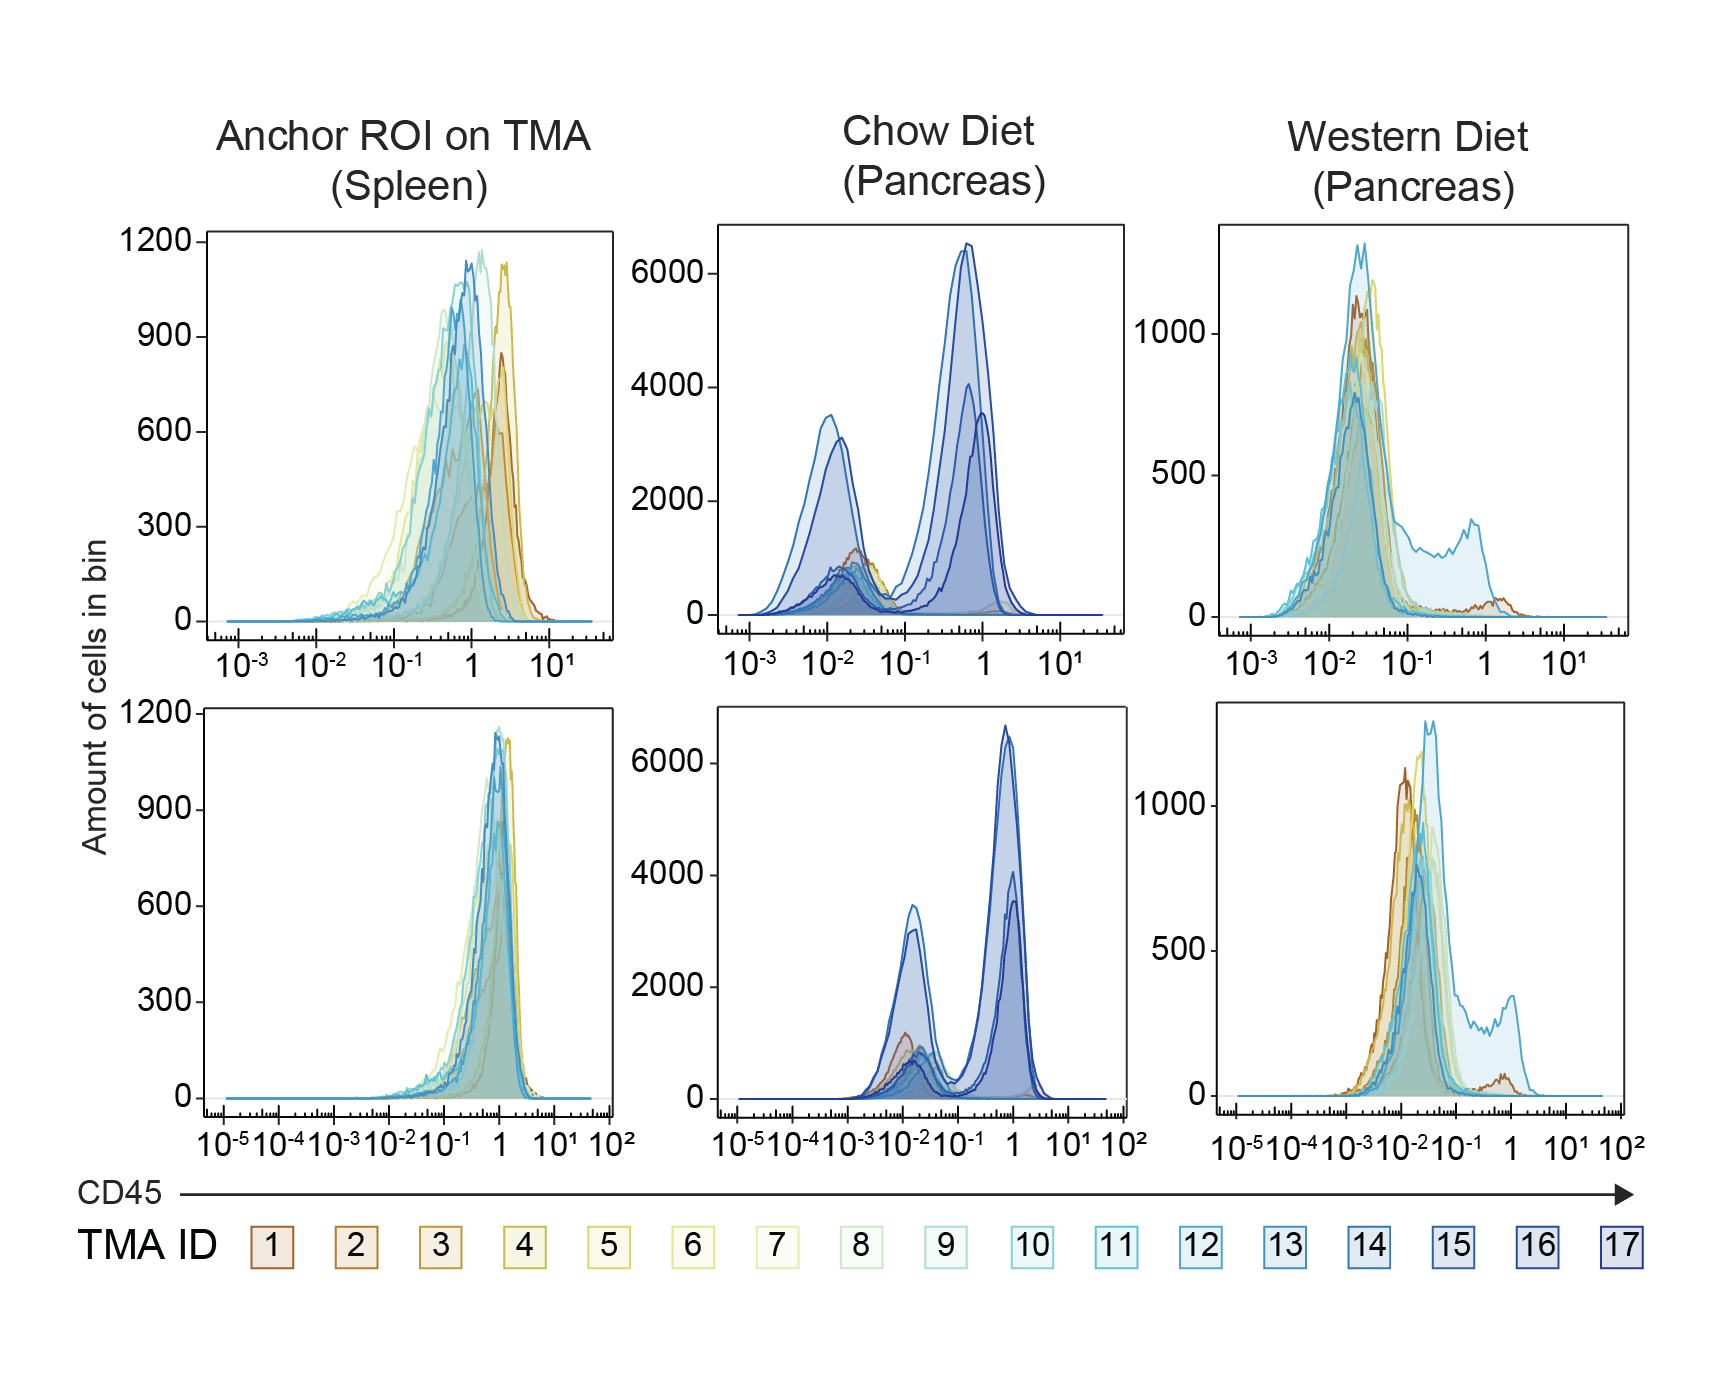
\includegraphics[width=\linewidth]{Appendix2/Fig/F2-A4-02.png}
% %     \caption[imc-anchor]{\textbf{Anchor and Batch Correction}}
% %     \label{suppl_fig:imc_anchor}
% % \end{figure}


% \begin{figure}[H]
%     \centering
%     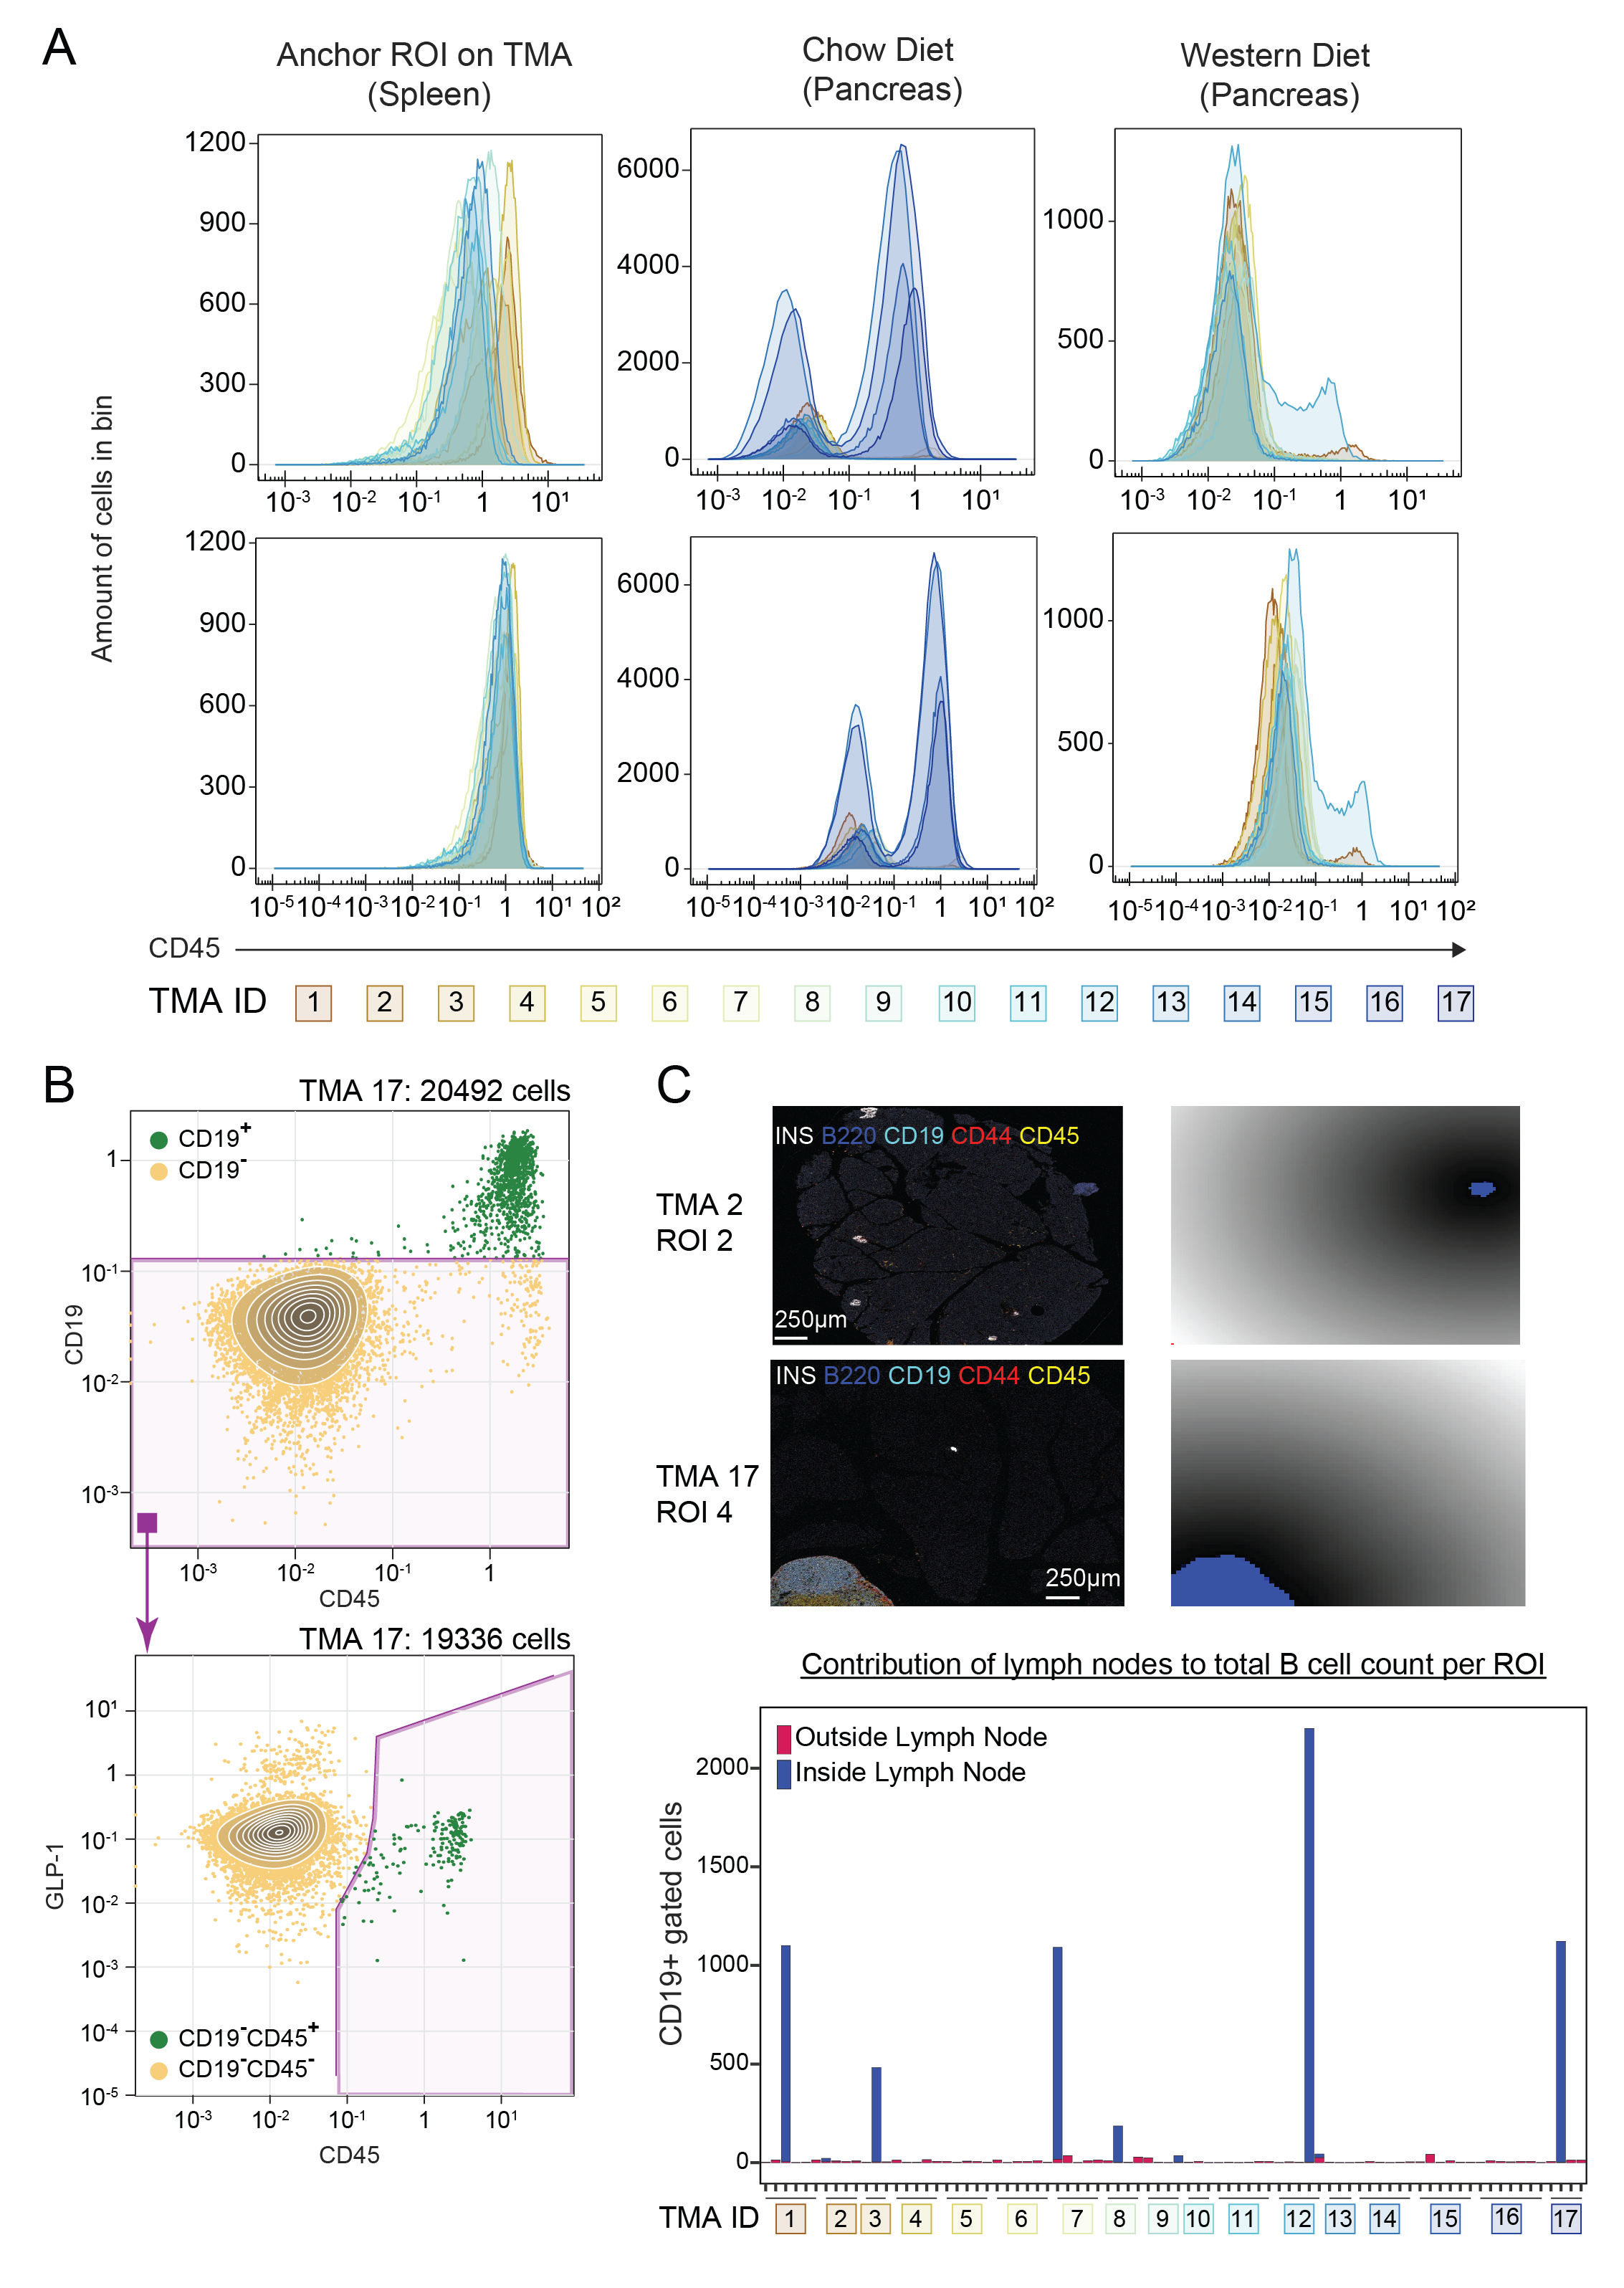
\includegraphics[width=14cm]{Appendix2/Fig/F2-A2-01.png}
%     \captionof{figure}[Exclusion of CD19\textsuperscript{+} B-cells]{\textbf{Exclusion of CD19+ B-cells}\\
%     \textbf{(A)} Histograms showing raw (top) and normalized (bottom) IMC signal intensity from the CD45 channel across all TMAs. The normalization process involved adjusting every channel across all TMAs relative to its positive peak intensity on the anchor Spleen ROI of the TMA (left column). \textbf{(B)} Representative scatter plots depicting the boolean gating strategy employed to identify pancreatic non-B-cell immune cells (CD19\textsuperscript{-}/CD45\textsuperscript{+}/GLP-1\textsuperscript{-}) within each TMA. \textbf{(C)} Representative ROIs showing two pancreatic lymph nodes (highlighted in blue, top left). Pancreatic lymph node masks were generated based on a composite overlay of signals from  B220, CD19, CD44, and CD45 (top right, see SI), scale bar, 250 µm. Bottom: Bar plot with counts of CD19\textsuperscript{+} B cells within and outside of tje generated lymph node masks.}
%     %[imc-anchorbcell]{\textbf{Exclusion of CD19+ B-cells}\\
%     %\textbf{(A)} Histograms showing raw (top) and normalized (bottom) IMC signal intensity from the CD45 channel across all TMAs. The normalization %process involved adjusting every channel across all TMAs relative to its positive peak intensity on the anchor Spleen ROI of the TMA (left column). \textbf{(B)} Representative scatter plots depicting the boolean gating strategy employed to identify pancreatic non-B-cell immune cells (CD19\textsuperscript{-}/CD45\textsuperscript{+}/GLP-1\textsuperscript{-}) within each TMA. \textbf{(C)} Representative ROIs showing two pancreatic lymph nodes (highlighted in blue, top left). Pancreatic lymph node masks were generated based on a composite overlay of signals from  B220, CD19, CD44, and CD45 (top right, see SI), scale bar, 250 µm. Bottom: Bar plot with counts of CD19\textsuperscript{+} B cells within and outside of tje generated lymph node masks.}
%     \label{suppl_fig:imc_anchorbcell}
% \end{figure}

% \begin{figure}[H]
%     \centering
%     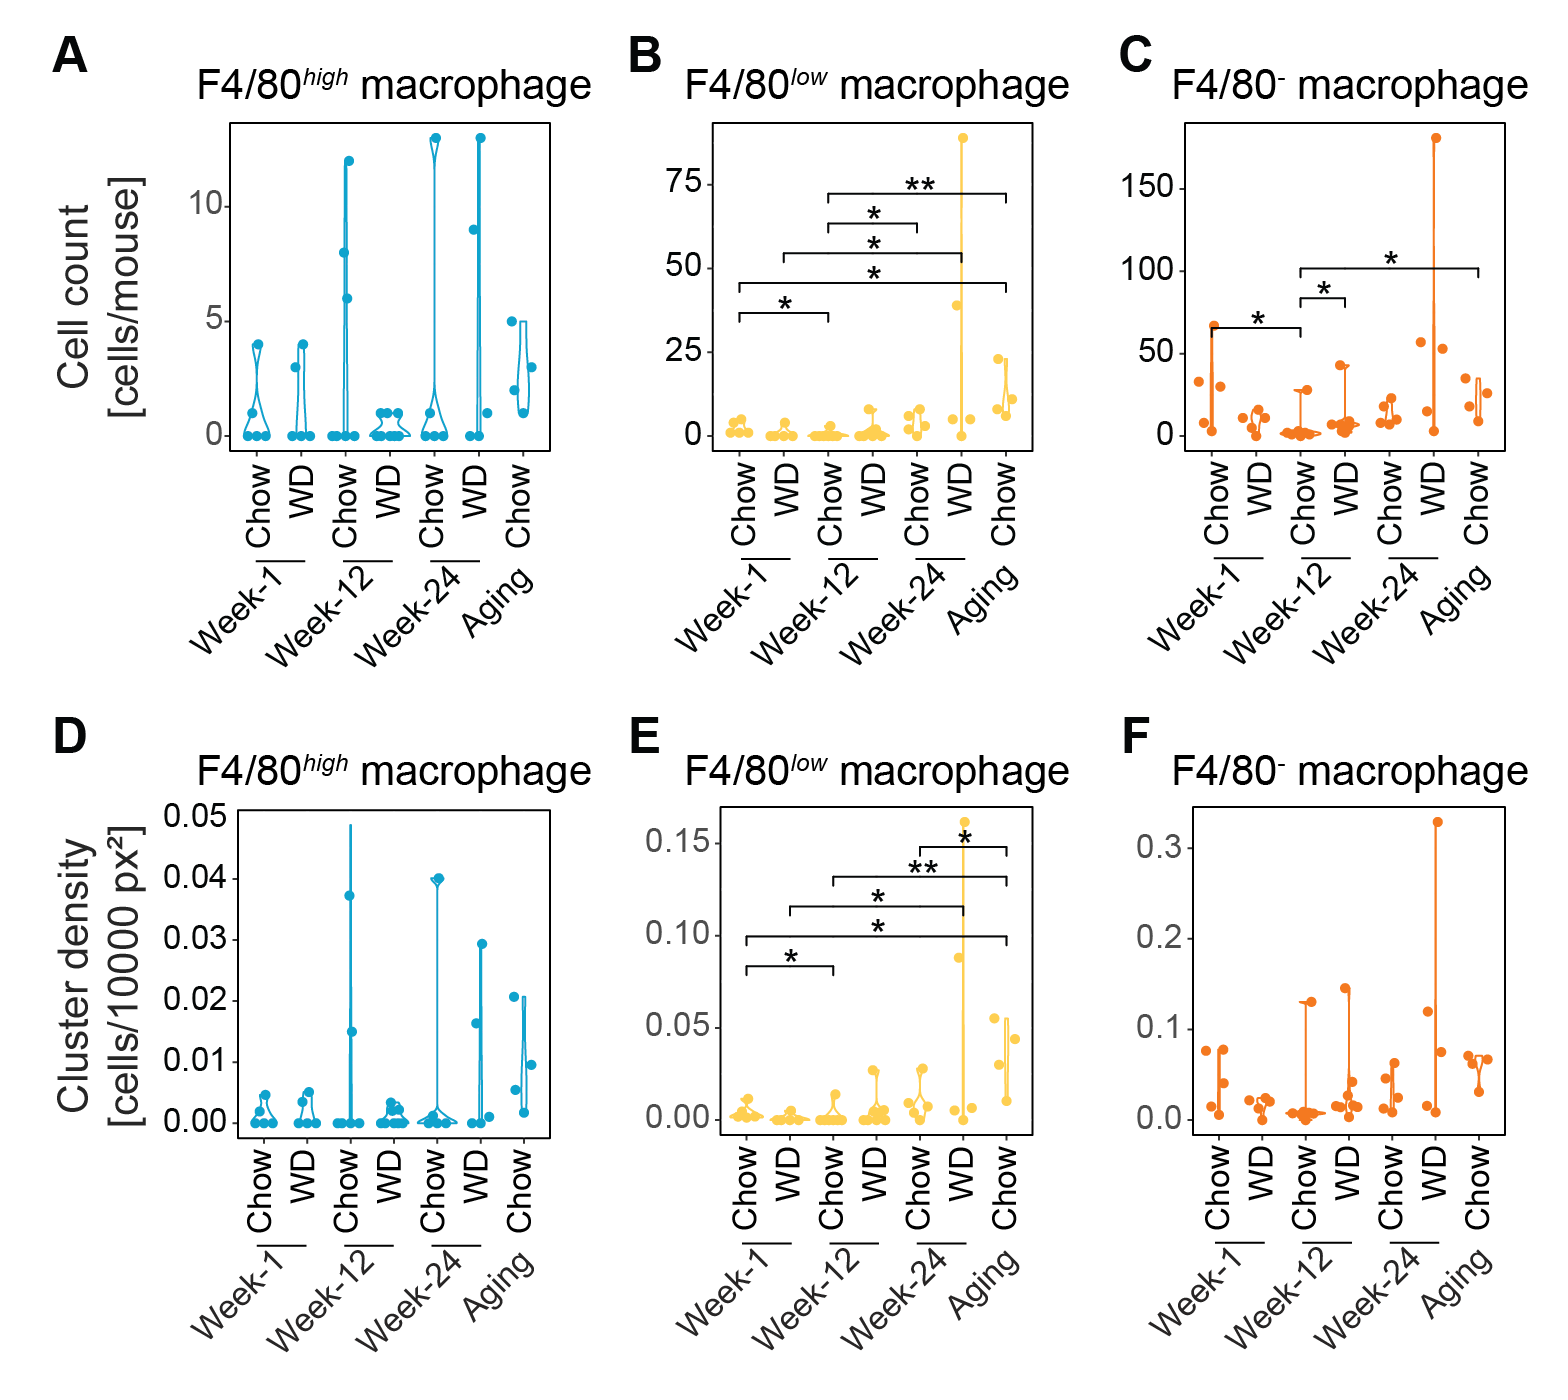
\includegraphics[width=\linewidth]{Appendix2/Fig/F2-A3-01.png}
%     \caption[Cell count and density of F4/80 macrophages from IMC analysis]{\textbf{Cell count and density of F4/80\textsuperscript{\textit{high}}, F4/80\textsuperscript{\textit{low}} and F4/80\textsuperscript{-} macrophage subtypes}\\
%     \textbf{(A-C)} Violin plots displaying the absolute counts of F4/80\textsuperscript{\textit{high}} \textbf{(A)}, F4/80\textsuperscript{\textit{low}} \textbf{(B)} and F4/80\textsuperscript{\textit{-}} \textbf{(C)} macrophages in non-lymph node pancreatic regions, presented for each mouse across various experimental conditions.  * p < 0.05, ** p < 0.01. p-values were calculated using the Wilcoxon rank-sum test. \textbf{(D-F)} Violin plots displaying the densities of F4/80\textsuperscript{\textit{high}} \textbf{(D)}, F4/80\textsuperscript{\textit{low}} \textbf{(E)} and F4/80\textsuperscript{\textit{-}} \textbf{(F)} macrophages in non-lymph node pancreatic regions, presented for each mouse across various experimental conditions. * p < 0.05, ** p < 0.01. p values were calculated using the Wilcoxon rank-sum test. }
%     \label{suppl_fig:imc_peri}
% \end{figure}


% \begin{figure}[H]
%     \centering
%     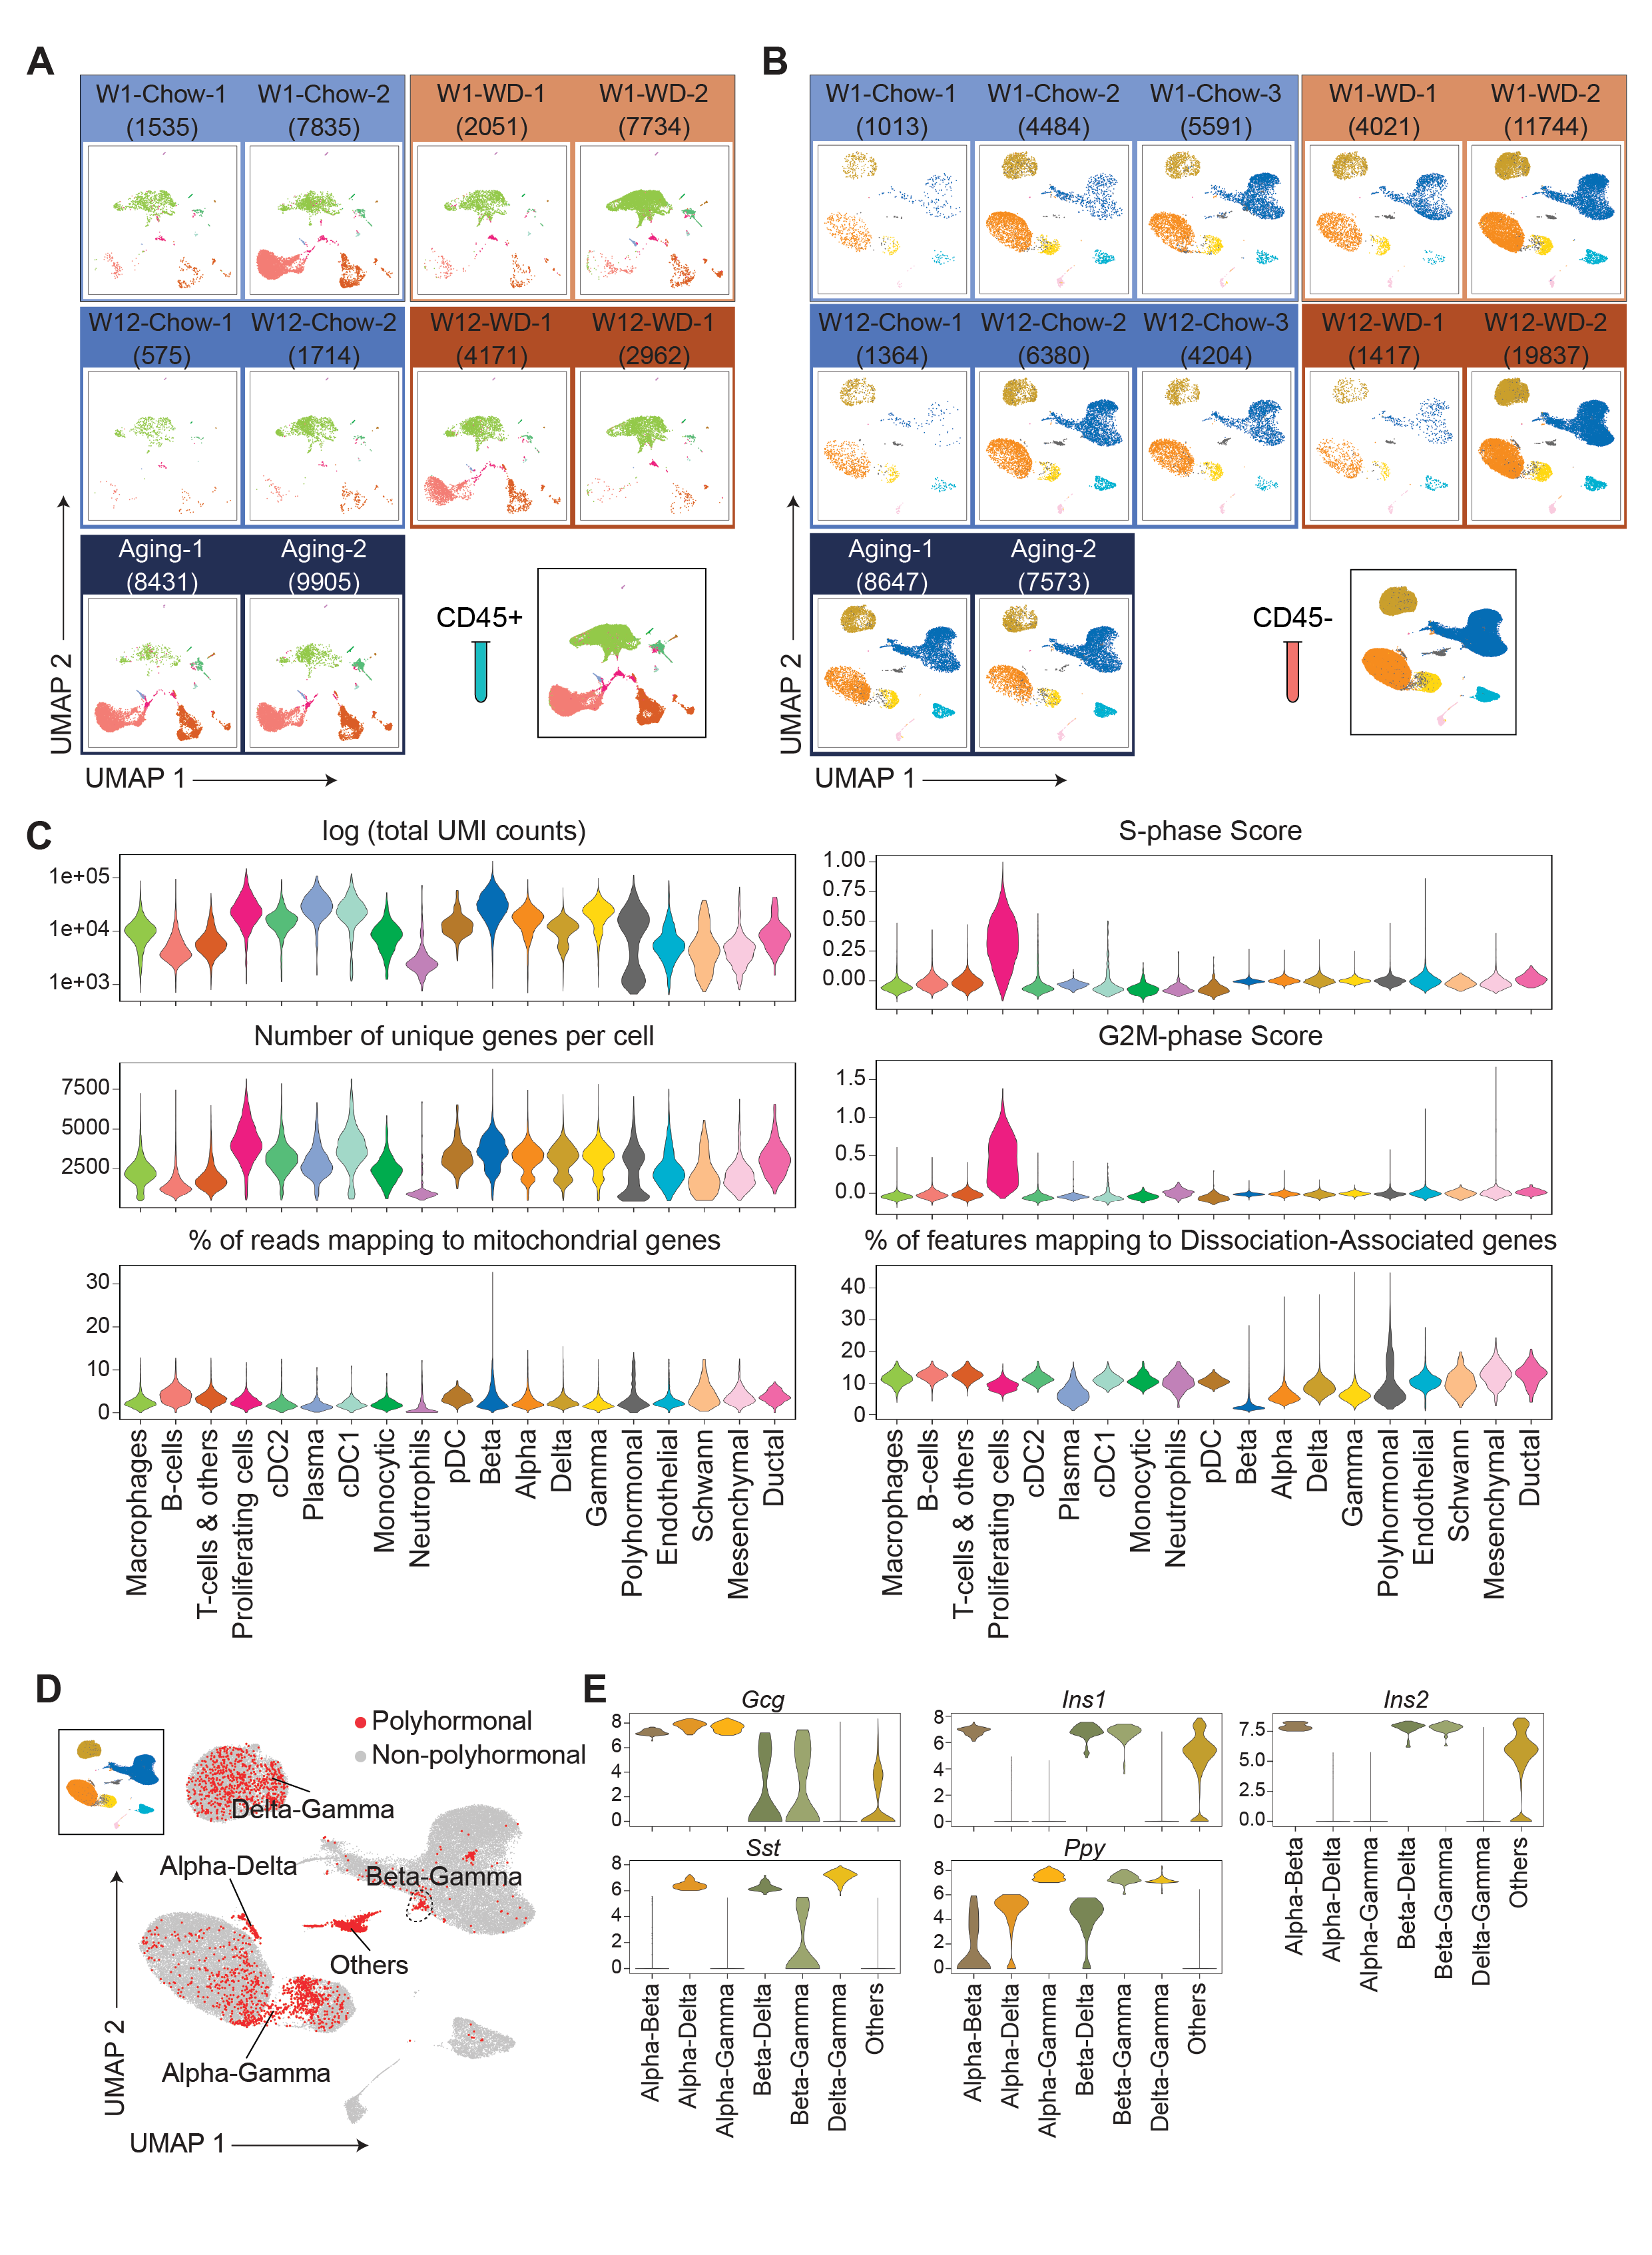
\includegraphics[width=13cm]{Appendix2/Fig/F2-A5-01.png}
%     \caption[suppl-fig:sc-qc]{\textbf{Quality control of scRNA-seq data}\\
%     \textbf{(A,B)} Split view of the CD45\textsuperscript{+} Immune cells (A) from \textbf{Fig.\ref{fig2-3} B} and CD45\textsuperscript{-} `Endocrine \& others’ cells (B) from \textbf{Fig.\ref{fig2-3} C} across all the sampled cohorts. The number of cells retained in each cohort post quality checks is indicated in parentheses. Chow-Cohort-3 for 1- and 12-weeks of feeding was dropped from the immune cell analysis prior to re-integration, as we did not perform immune cell enrichment using FACS for this cohort. \textbf{(C)} Violin plots of QC metrics for every annotated cell-type after integration – logarithm of UMI counts per cell (top left); number of unique features per cell (middle left); percentage of reads mapping to mitochondrial genome (bottom left); cell-cycle phase scores (top and middle right) - These metrices did not dictate the clustering and subsequent annotation of the integrated data. In addition to standard QC metrics, we also examined known gene features induced by enzymatic dissociation (bottom-right) \textbf{(D)} UMAP embedding of Endocrine \& Others' from \textbf{Fig.\ref{fig2-3} C} depicting the identified polyhormonal populations (in red). The non-polyhormonal cells are depicted in grey. The \textbf{(E)} Violin plots of the five primary islet hormone markers across the identified polyhormonal populations in \textbf{(A)}}
%     \label{suppl_fig:sc_qc}
% \end{figure}

% \begin{figure}[H]
%     \centering
%     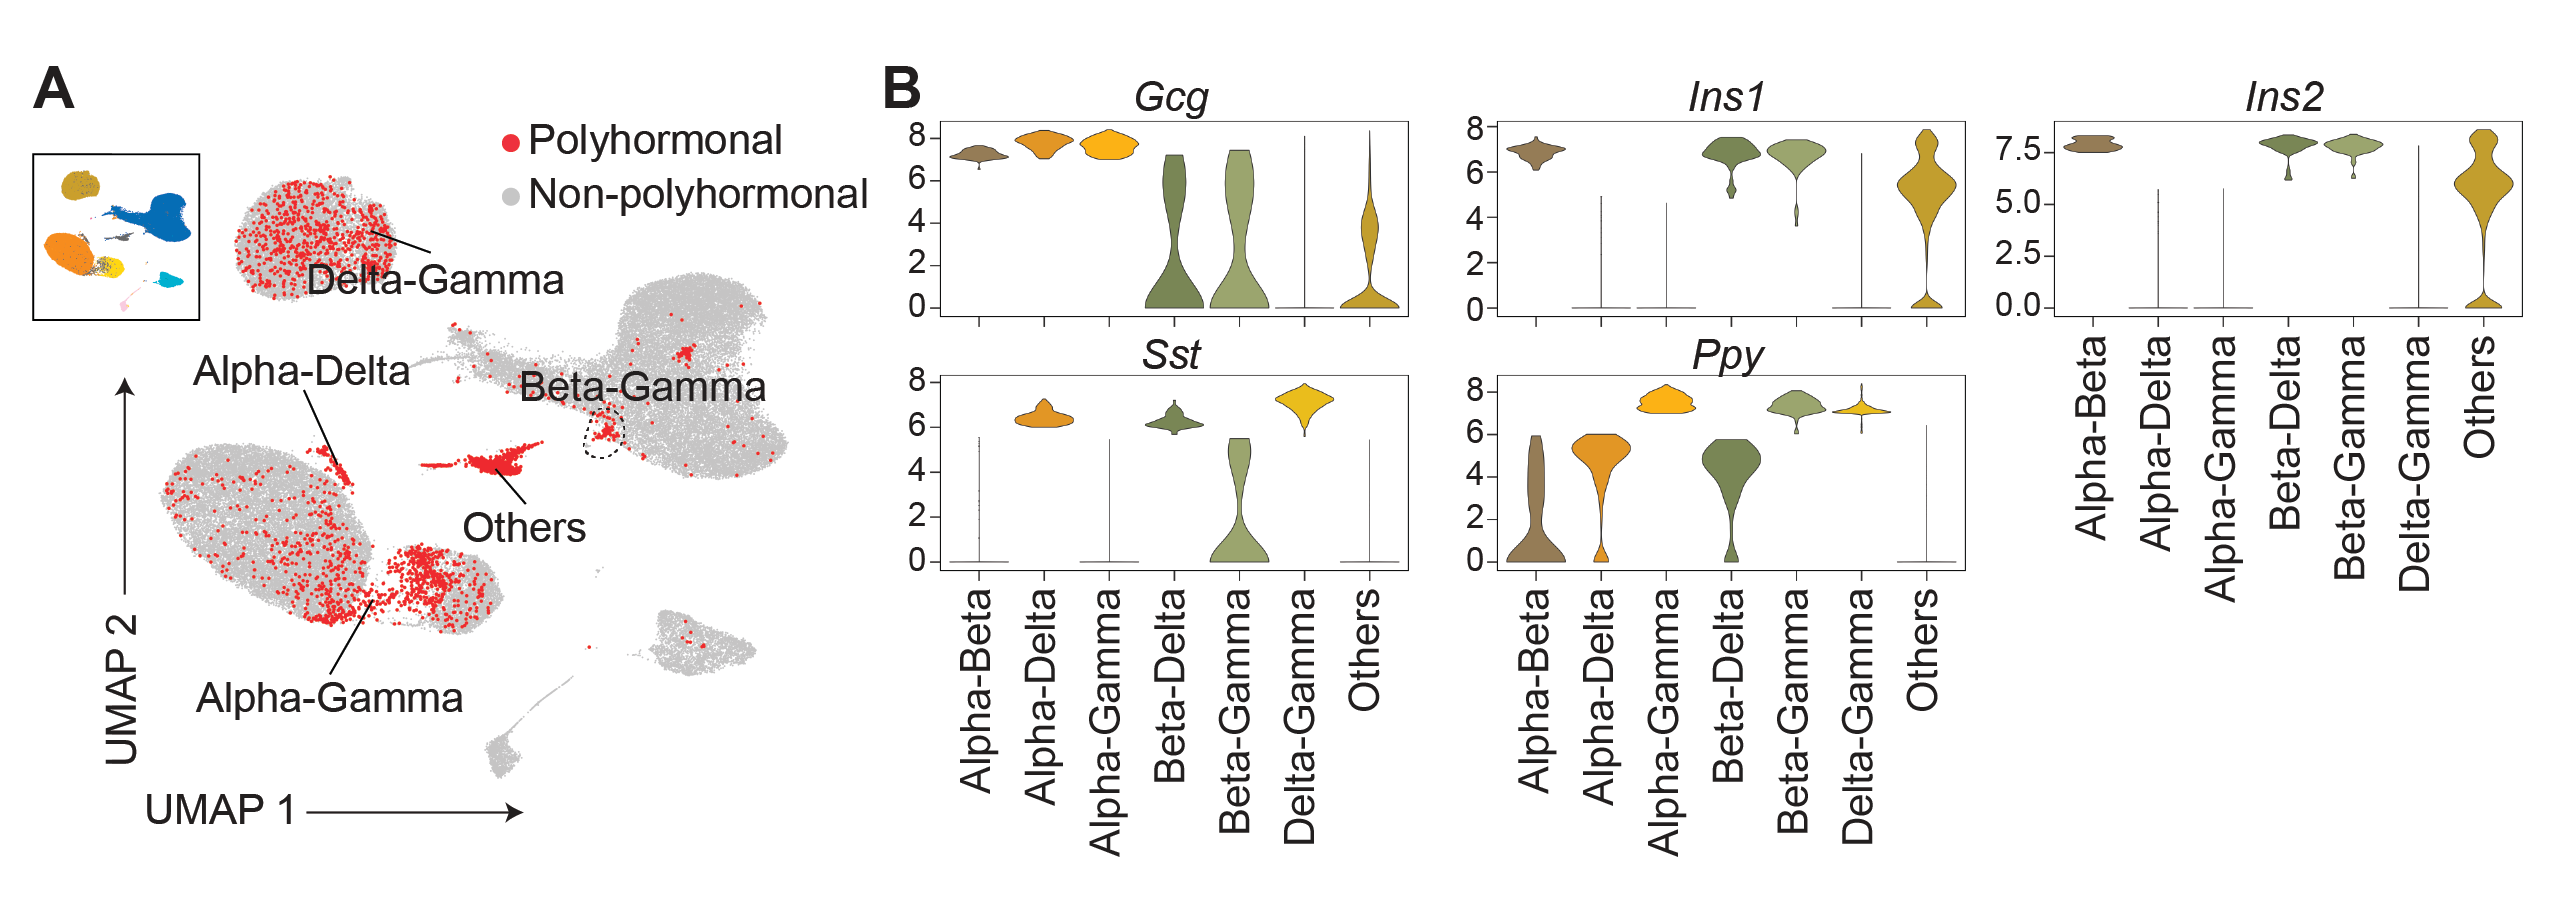
\includegraphics[width=\linewidth]{Appendix2/Fig/F2-A6-01.png}
%     \caption[suppl-fig:sc-endo]{\textbf{Annotating Polyhormonal cells}\\
%     \textbf{(A)} UMAP embedding of Endocrine \& Others' from \textbf{Fig.\ref{fig2-3} C} depicting the identified polyhormonal populations (in red). The non-polyhormonal cells are depicted in grey. The \textbf{(B)} Violin plots of the five primary islet hormone markers across the identified polyhormonal populations in \textbf{(A)}}
%     \label{suppl_fig:sc_endo}
% \end{figure}

% \begin{figure}[H]
%     \centering
%     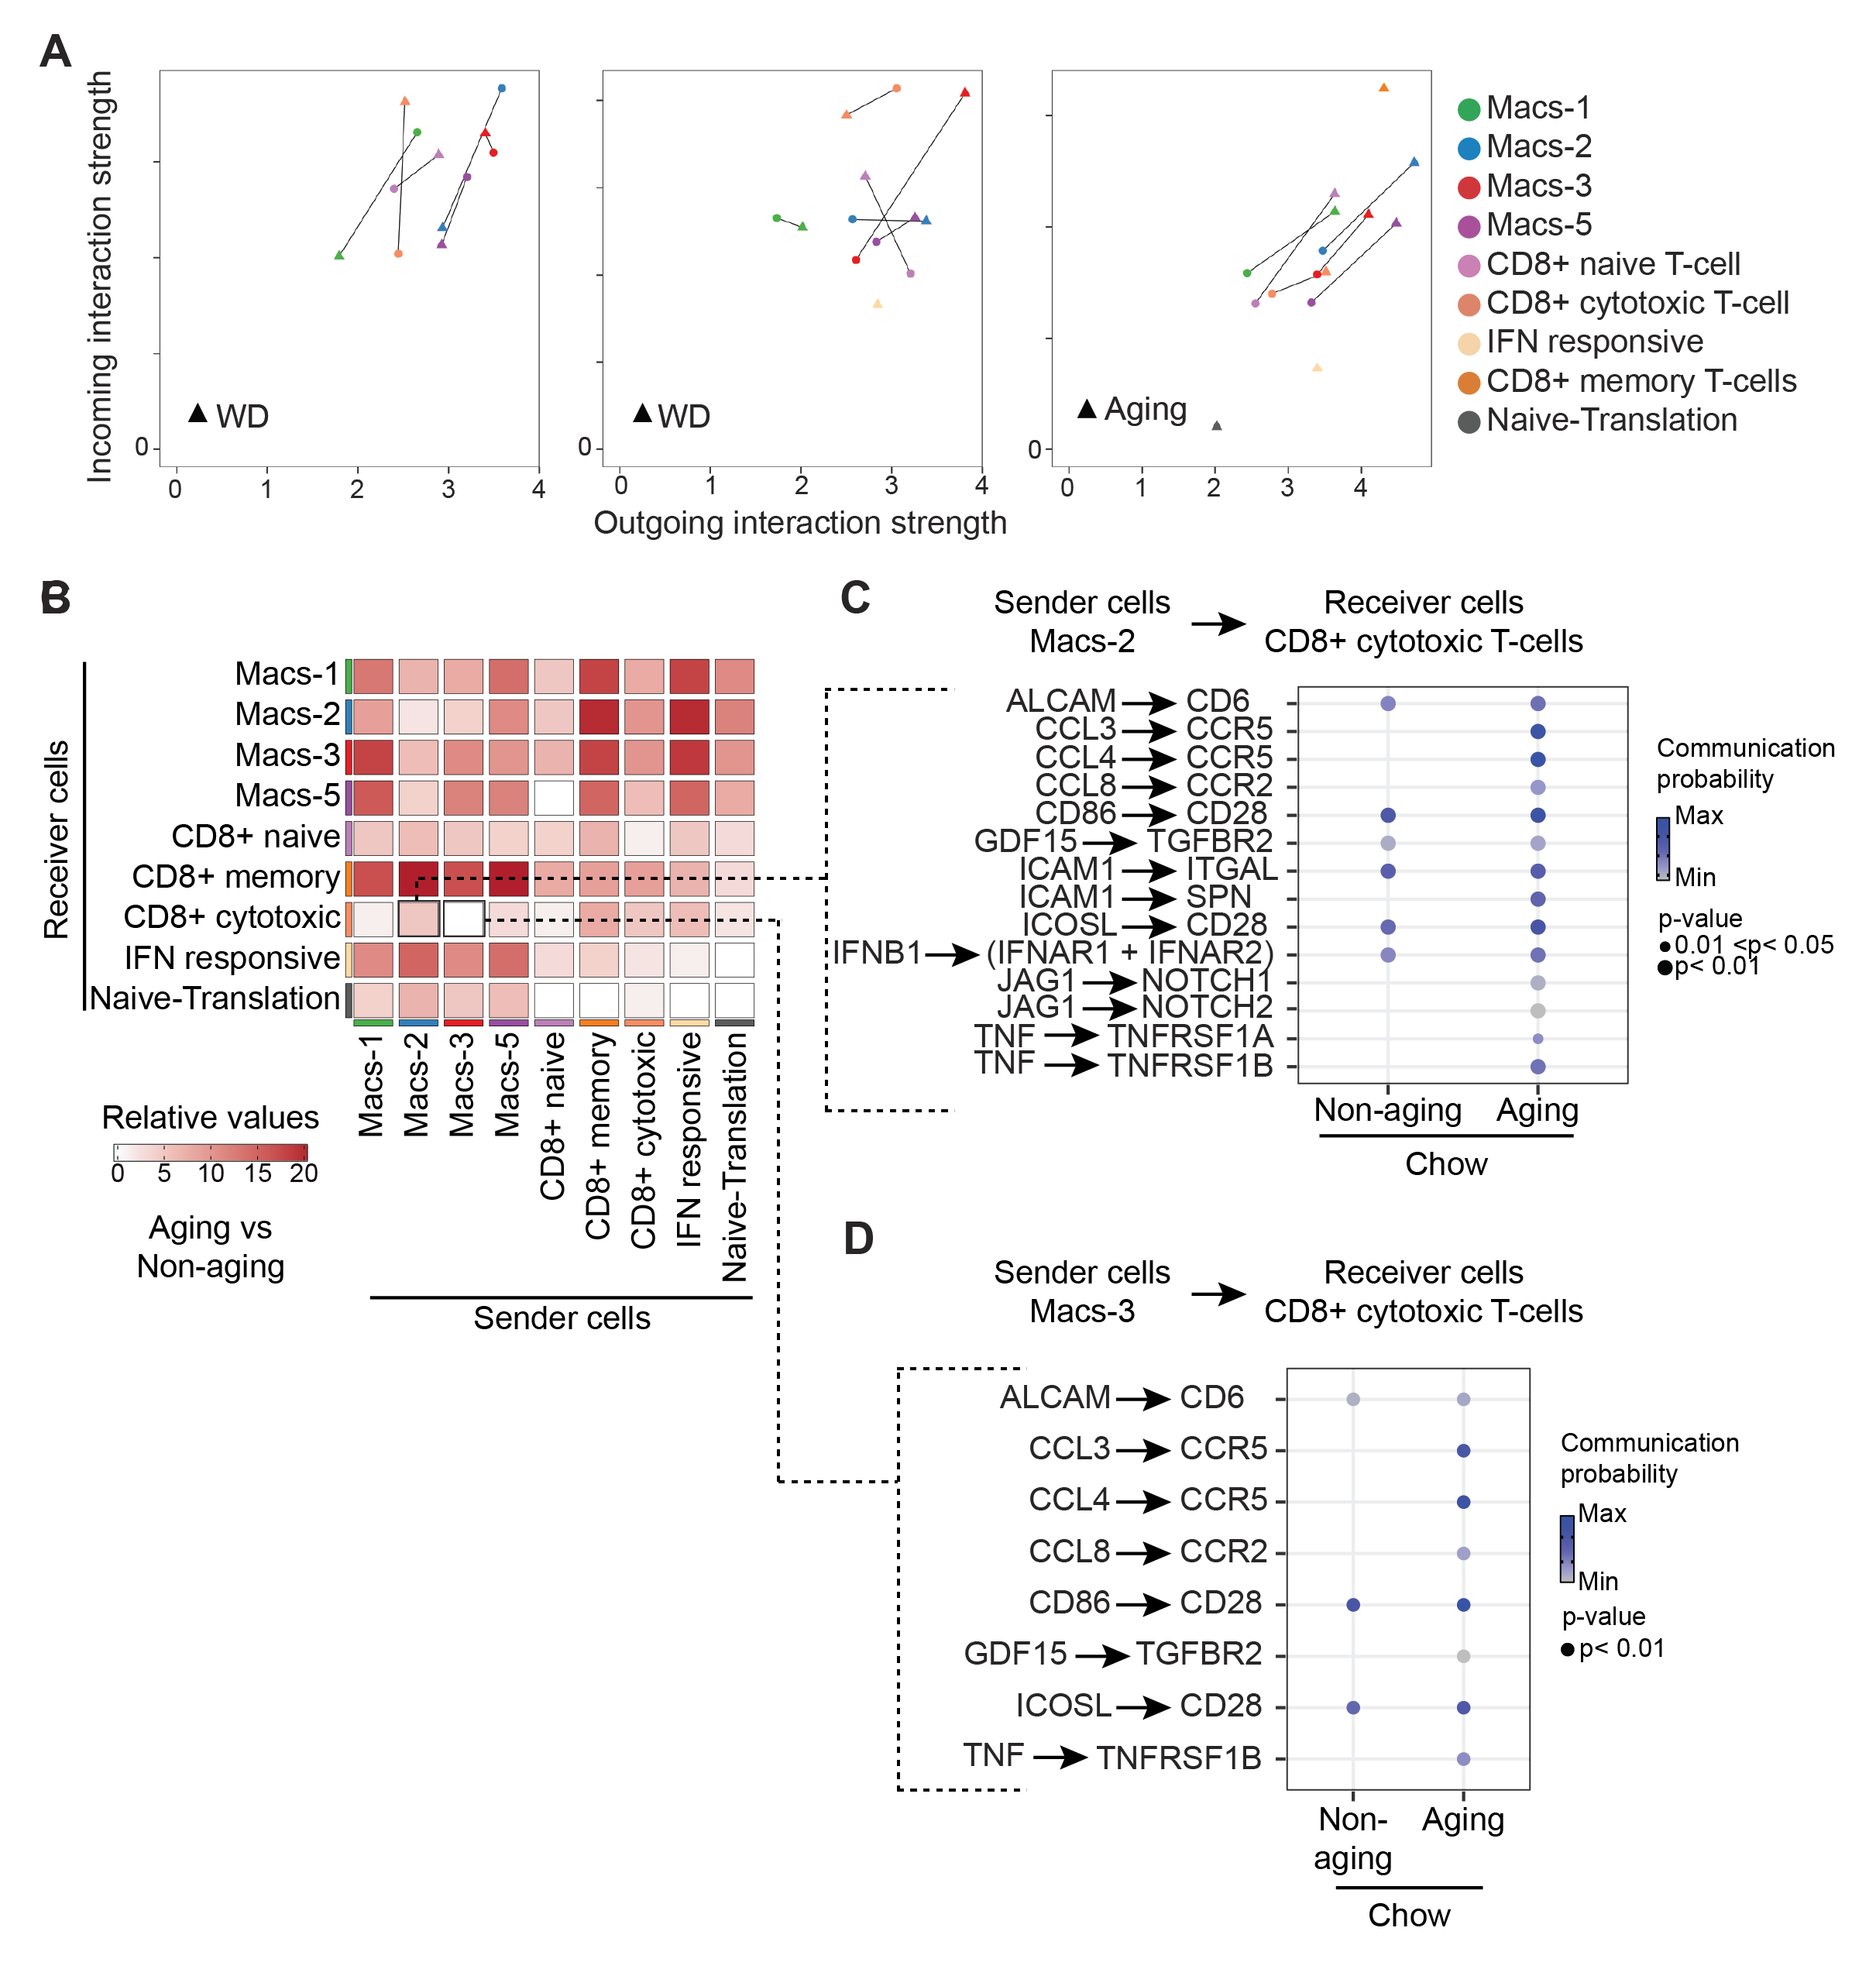
\includegraphics[width=\linewidth]{Appendix2/Fig/F2-A1-01.png}
%     \caption[suppl-fig:cell-cell1]{\textbf{Ligand-receptor analysis in islet resident immune cells }\\
%     \textbf{(A)} Scatter plot depicting the outgoing interaction strength (on X-axis) and the incoming interaction strength (on Y-axis) for the indicated cell populations at Week-1 Chow (n=3) and Week-1 WD (n=2) (left), Weeks-12 Chow (n=3) and Weeks-12 WD (n=2) (middle) and Aging (n=2) and Non-Aging (right) time-points. The Non-Aging group is comprised of Week-1 (n=3) and Week-12 (n=3) Chow diet cohorts. \textbf{(B)} Heatmap depicting differential number of interactions in the Aging cohort (n = 2) compared to the Non-Aging (Week-1 Chow (n=3) and Week-12 Chow (n=3)) cohorts between the indicated cell populations. \textbf{(C)}Dot plots depicting ligand-receptor interaction intensity, with signals from Macs-2 to CD8+ cytotoxic, under Chow (n=3) and one-week post-Western diet (n=2) conditions. The plots specifically highlight signals that exhibit an increase in interaction intensity from non-aging to aging condition. The dot color and size represent the calculated communication probability and p-values. p-values are computed from one-sided permutation test directly within CellChat. \textbf{(C)} Dot plots depicting ligand-receptor interaction intensity, with signals from Macs-3 to CD8+ cytotoxic, under Chow (n=3) and one-week post-Western diet (n=2) conditions. The plots specifically highlight signals that exhibit an increase in interaction intensity from non-aging to aging condition. The dot color and size represent the calculated communication probability and p-values. p-values are computed from one-sided permutation test directly within CellChat.}
%     \label{suppl_fig:cell_cell1}
% \end{figure}

% % \begin{figure}[!t]
% %     \centering
% %     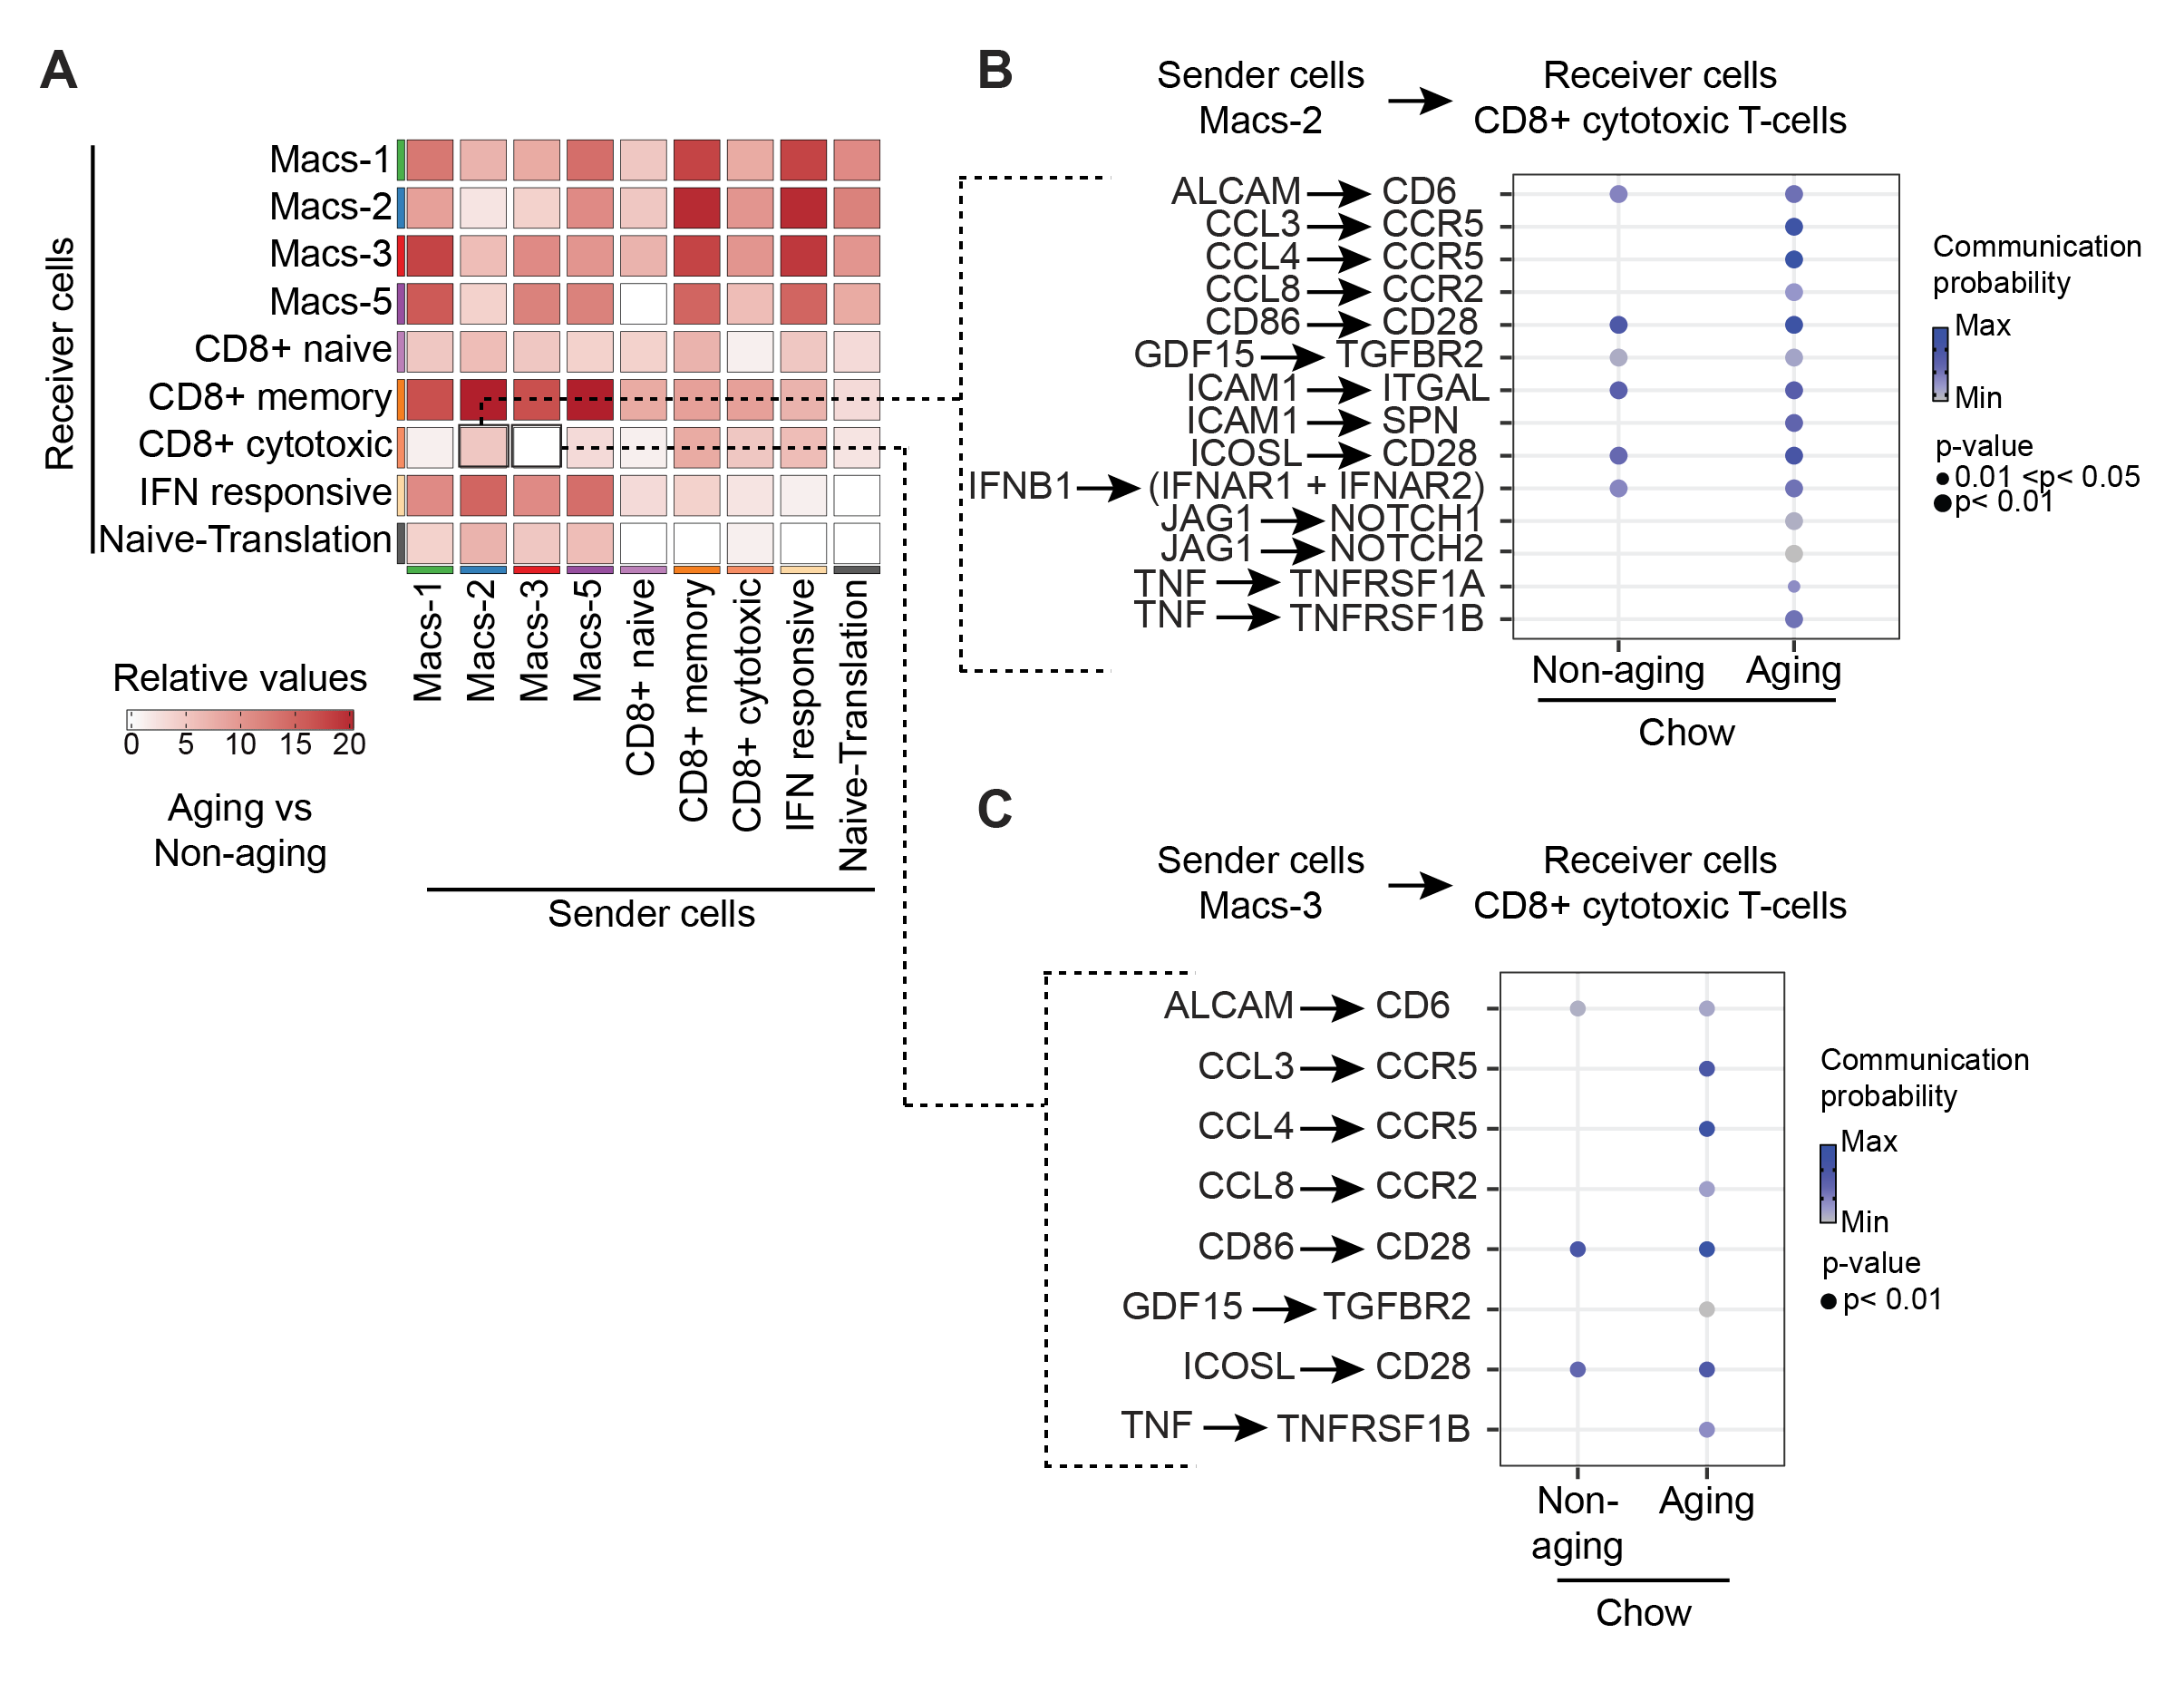
\includegraphics[width=\linewidth]{Appendix2/Fig/F2-A1-02.png}
% %     \caption[Differential interaction analysis between chow-fed aging and chow-fed non-aging (Week-1 and Weeks-12) groups]{\textbf{Differential interaction analysis between chow-fed aging and chow-fed non-aging (Week-1 and Weeks-12) groups}\\\\
% %     \textbf{(A)} Heatmap depicting differential number of interactions in the Aging cohort (n = 2) compared to the Non-Aging (Week-1 Chow (n=3) and Week-12 Chow (n=3)) cohorts between the indicated cell populations. \textbf{(B)}Dot plots depicting ligand-receptor interaction intensity, with signals from Macs-2 to CD8+ cytotoxic, under Chow (n=3) and one-week post-Western diet (n=2) conditions. The plots specifically highlight signals that exhibit an increase in interaction intensity from non-aging to aging condition. The dot color and size represent the calculated communication probability and p-values. p-values are computed from one-sided permutation test directly within CellChat. \textbf{(C)} Dot plots depicting ligand-receptor interaction intensity, with signals from Macs-3 to CD8+ cytotoxic, under Chow (n=3) and one-week post-Western diet (n=2) conditions. The plots specifically highlight signals that exhibit an increase in interaction intensity from non-aging to aging condition. The dot color and size represent the calculated communication probability and p-values. p-values are computed from one-sided permutation test directly within CellChat.}
% %     \label{suppl_fig:cell_cell2}
% % \end{figure}


\section{Additional results for Chapter 3}

\begin{figure}[H]
\centering
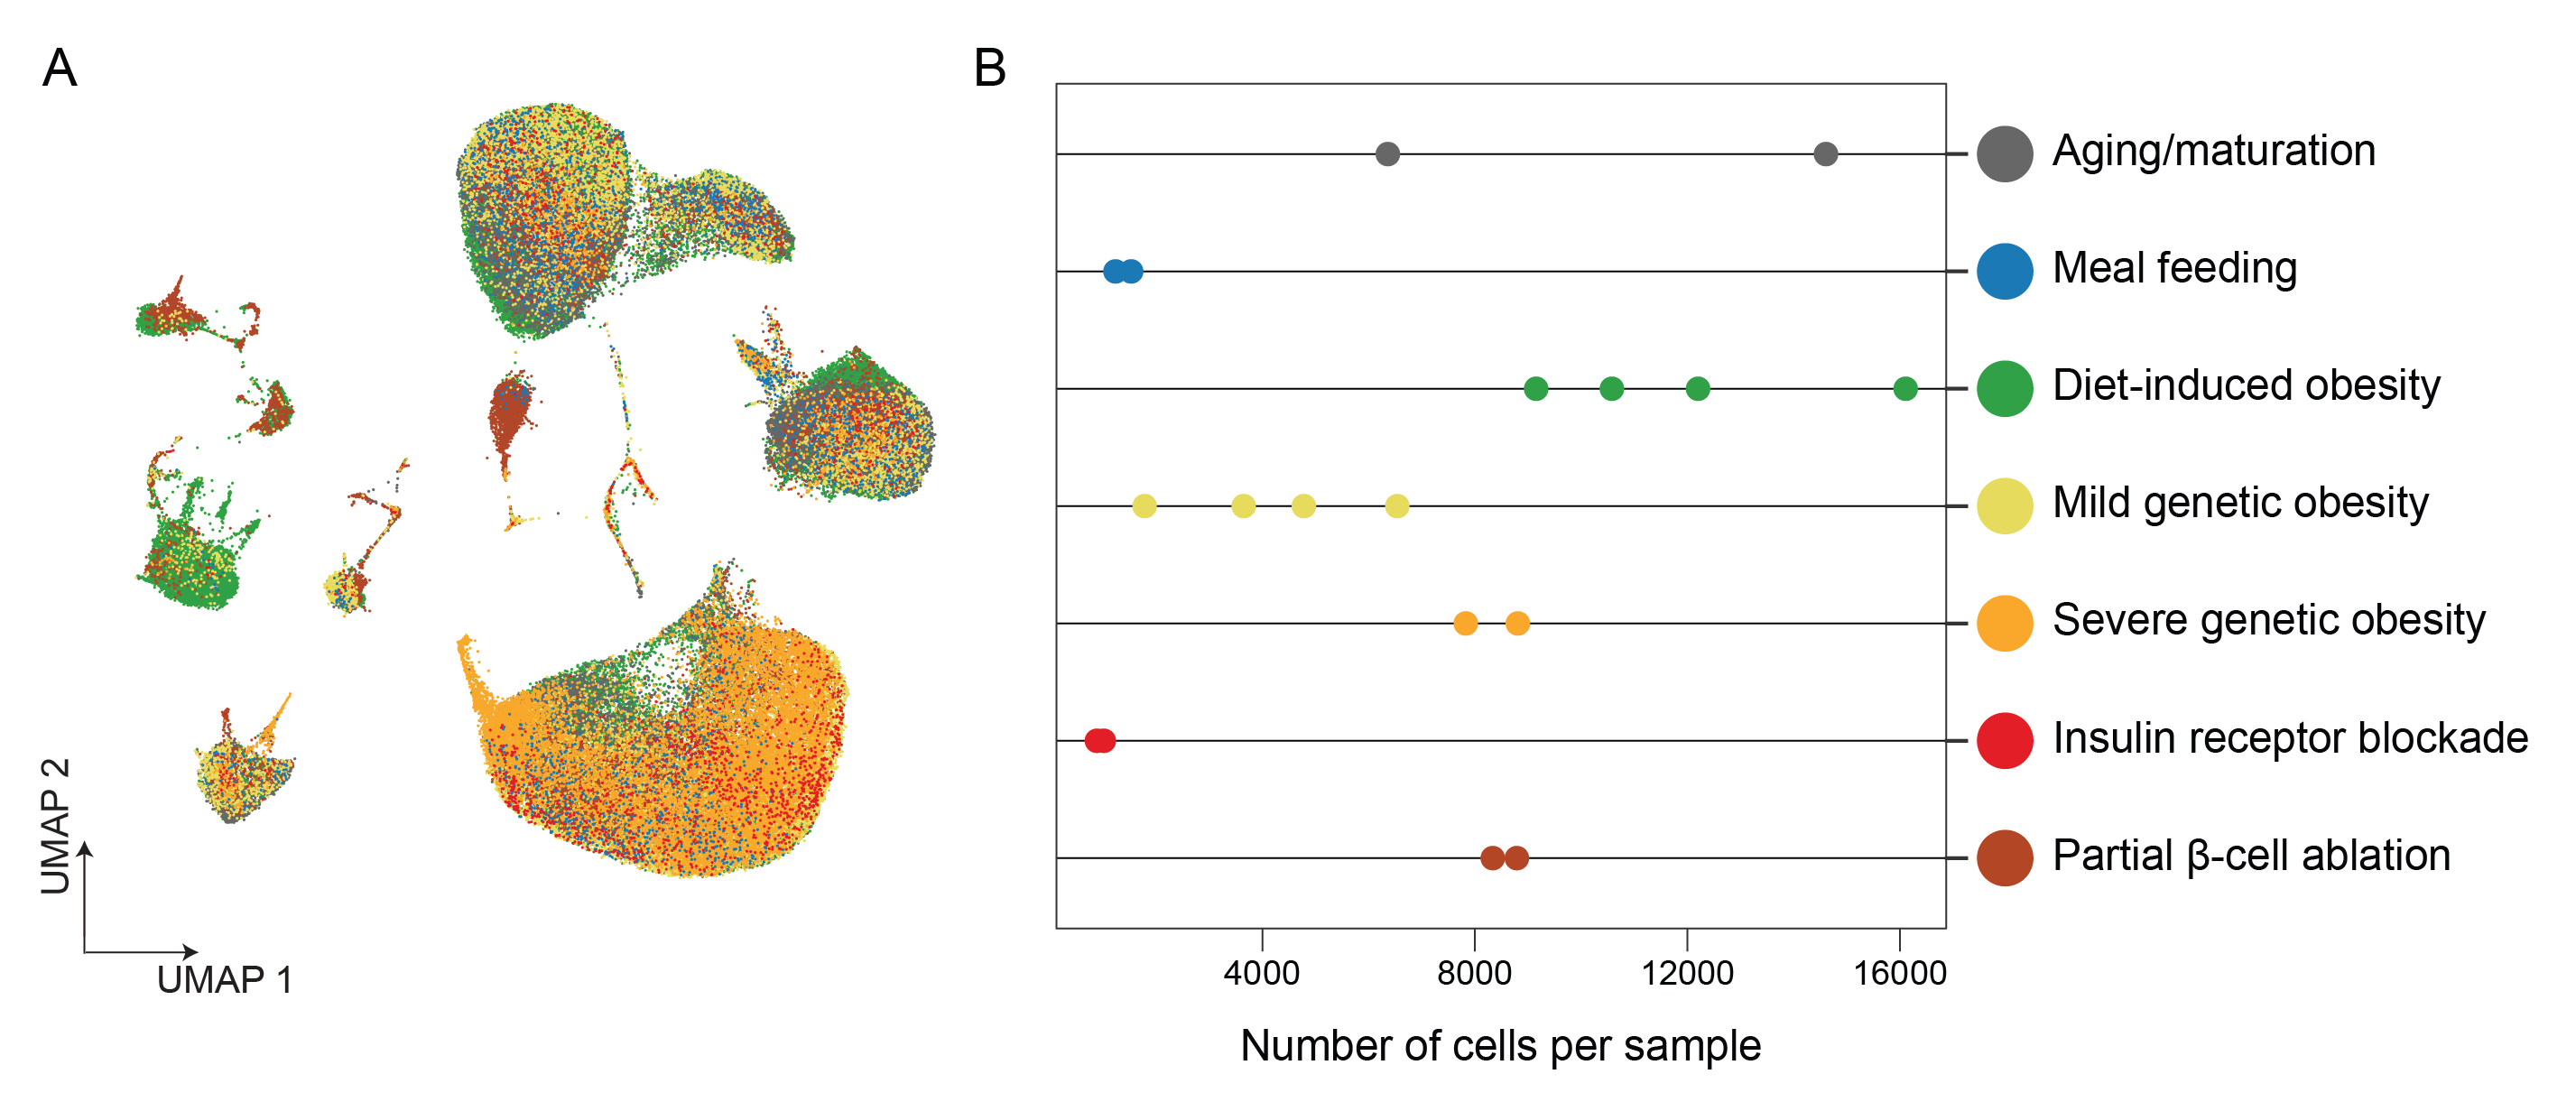
\includegraphics[width=\linewidth]{Appendix2/Fig/F3-2-v2-02.png}
\caption[Study distribution within the full integrated data]{\textbf{Study distribution within the full integrated data}}
\label{suppl_fig:chp3_study}
\end{figure}

% \begin{figure}[H]
% \centering
% 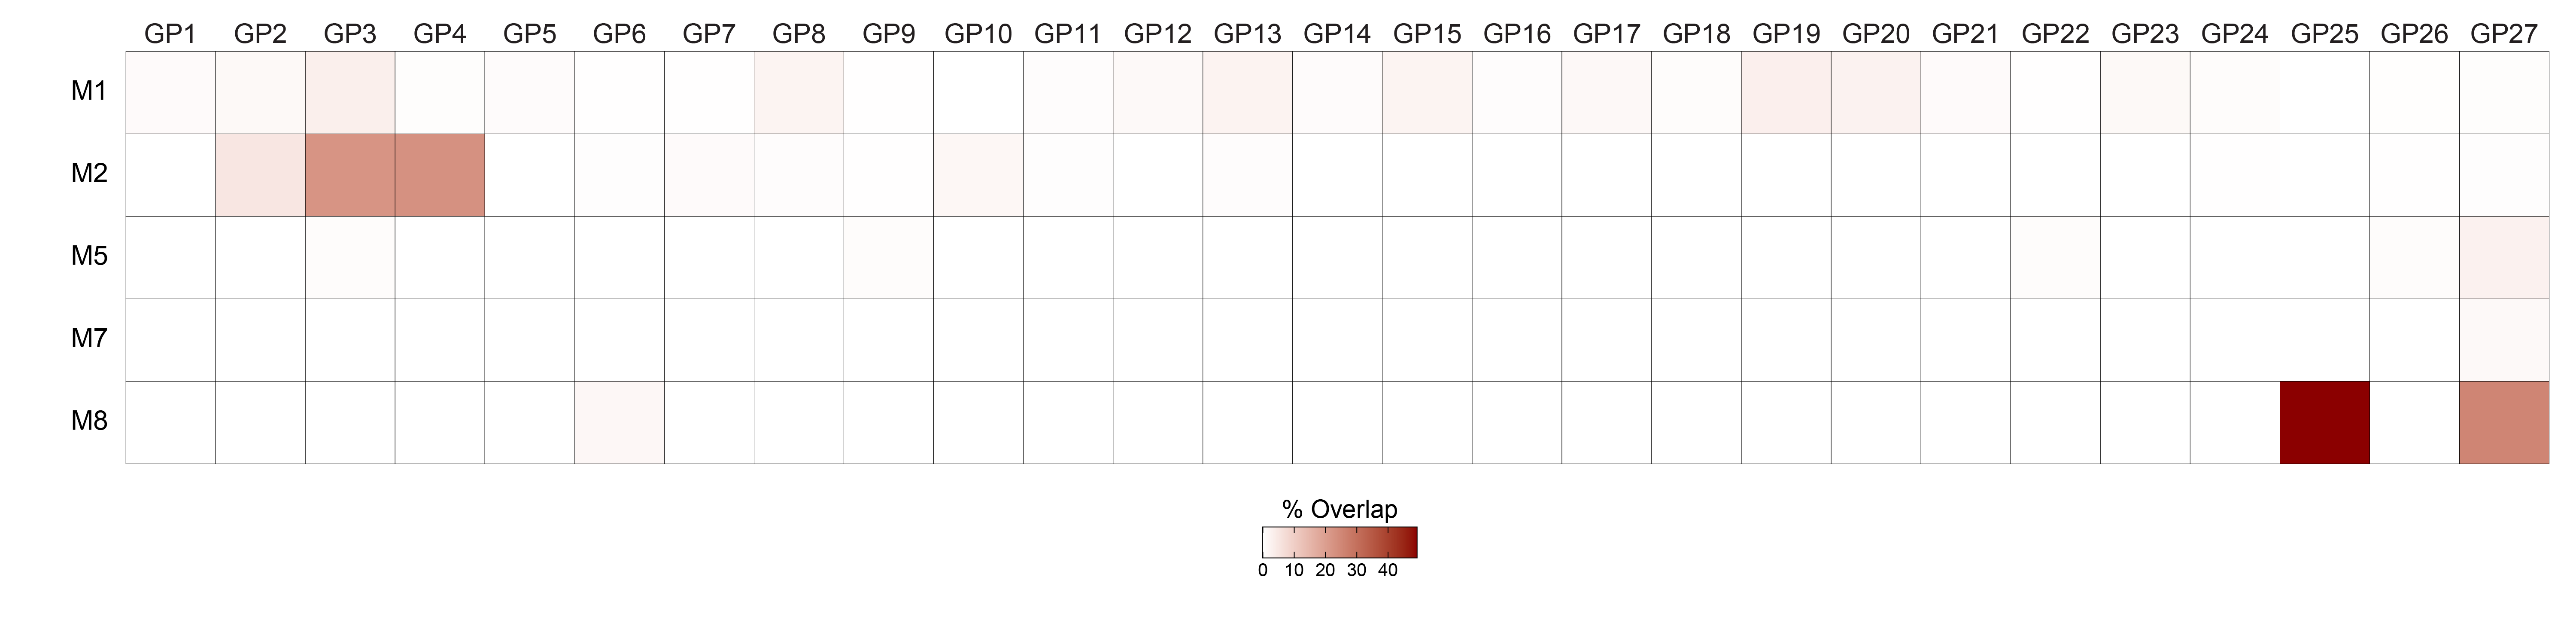
\includegraphics[width=\linewidth]{Appendix2/Fig/F3-5-01.png}
% \caption[Overlap between gene modules identified in this study and gene programs from MIA]{\textbf{Overlap between gene modules identified in this study and gene programs from MIA}}
% \label{suppl_fig:chp3_overlap}
% \end{figure}



\begin{figure}[H]
\centering
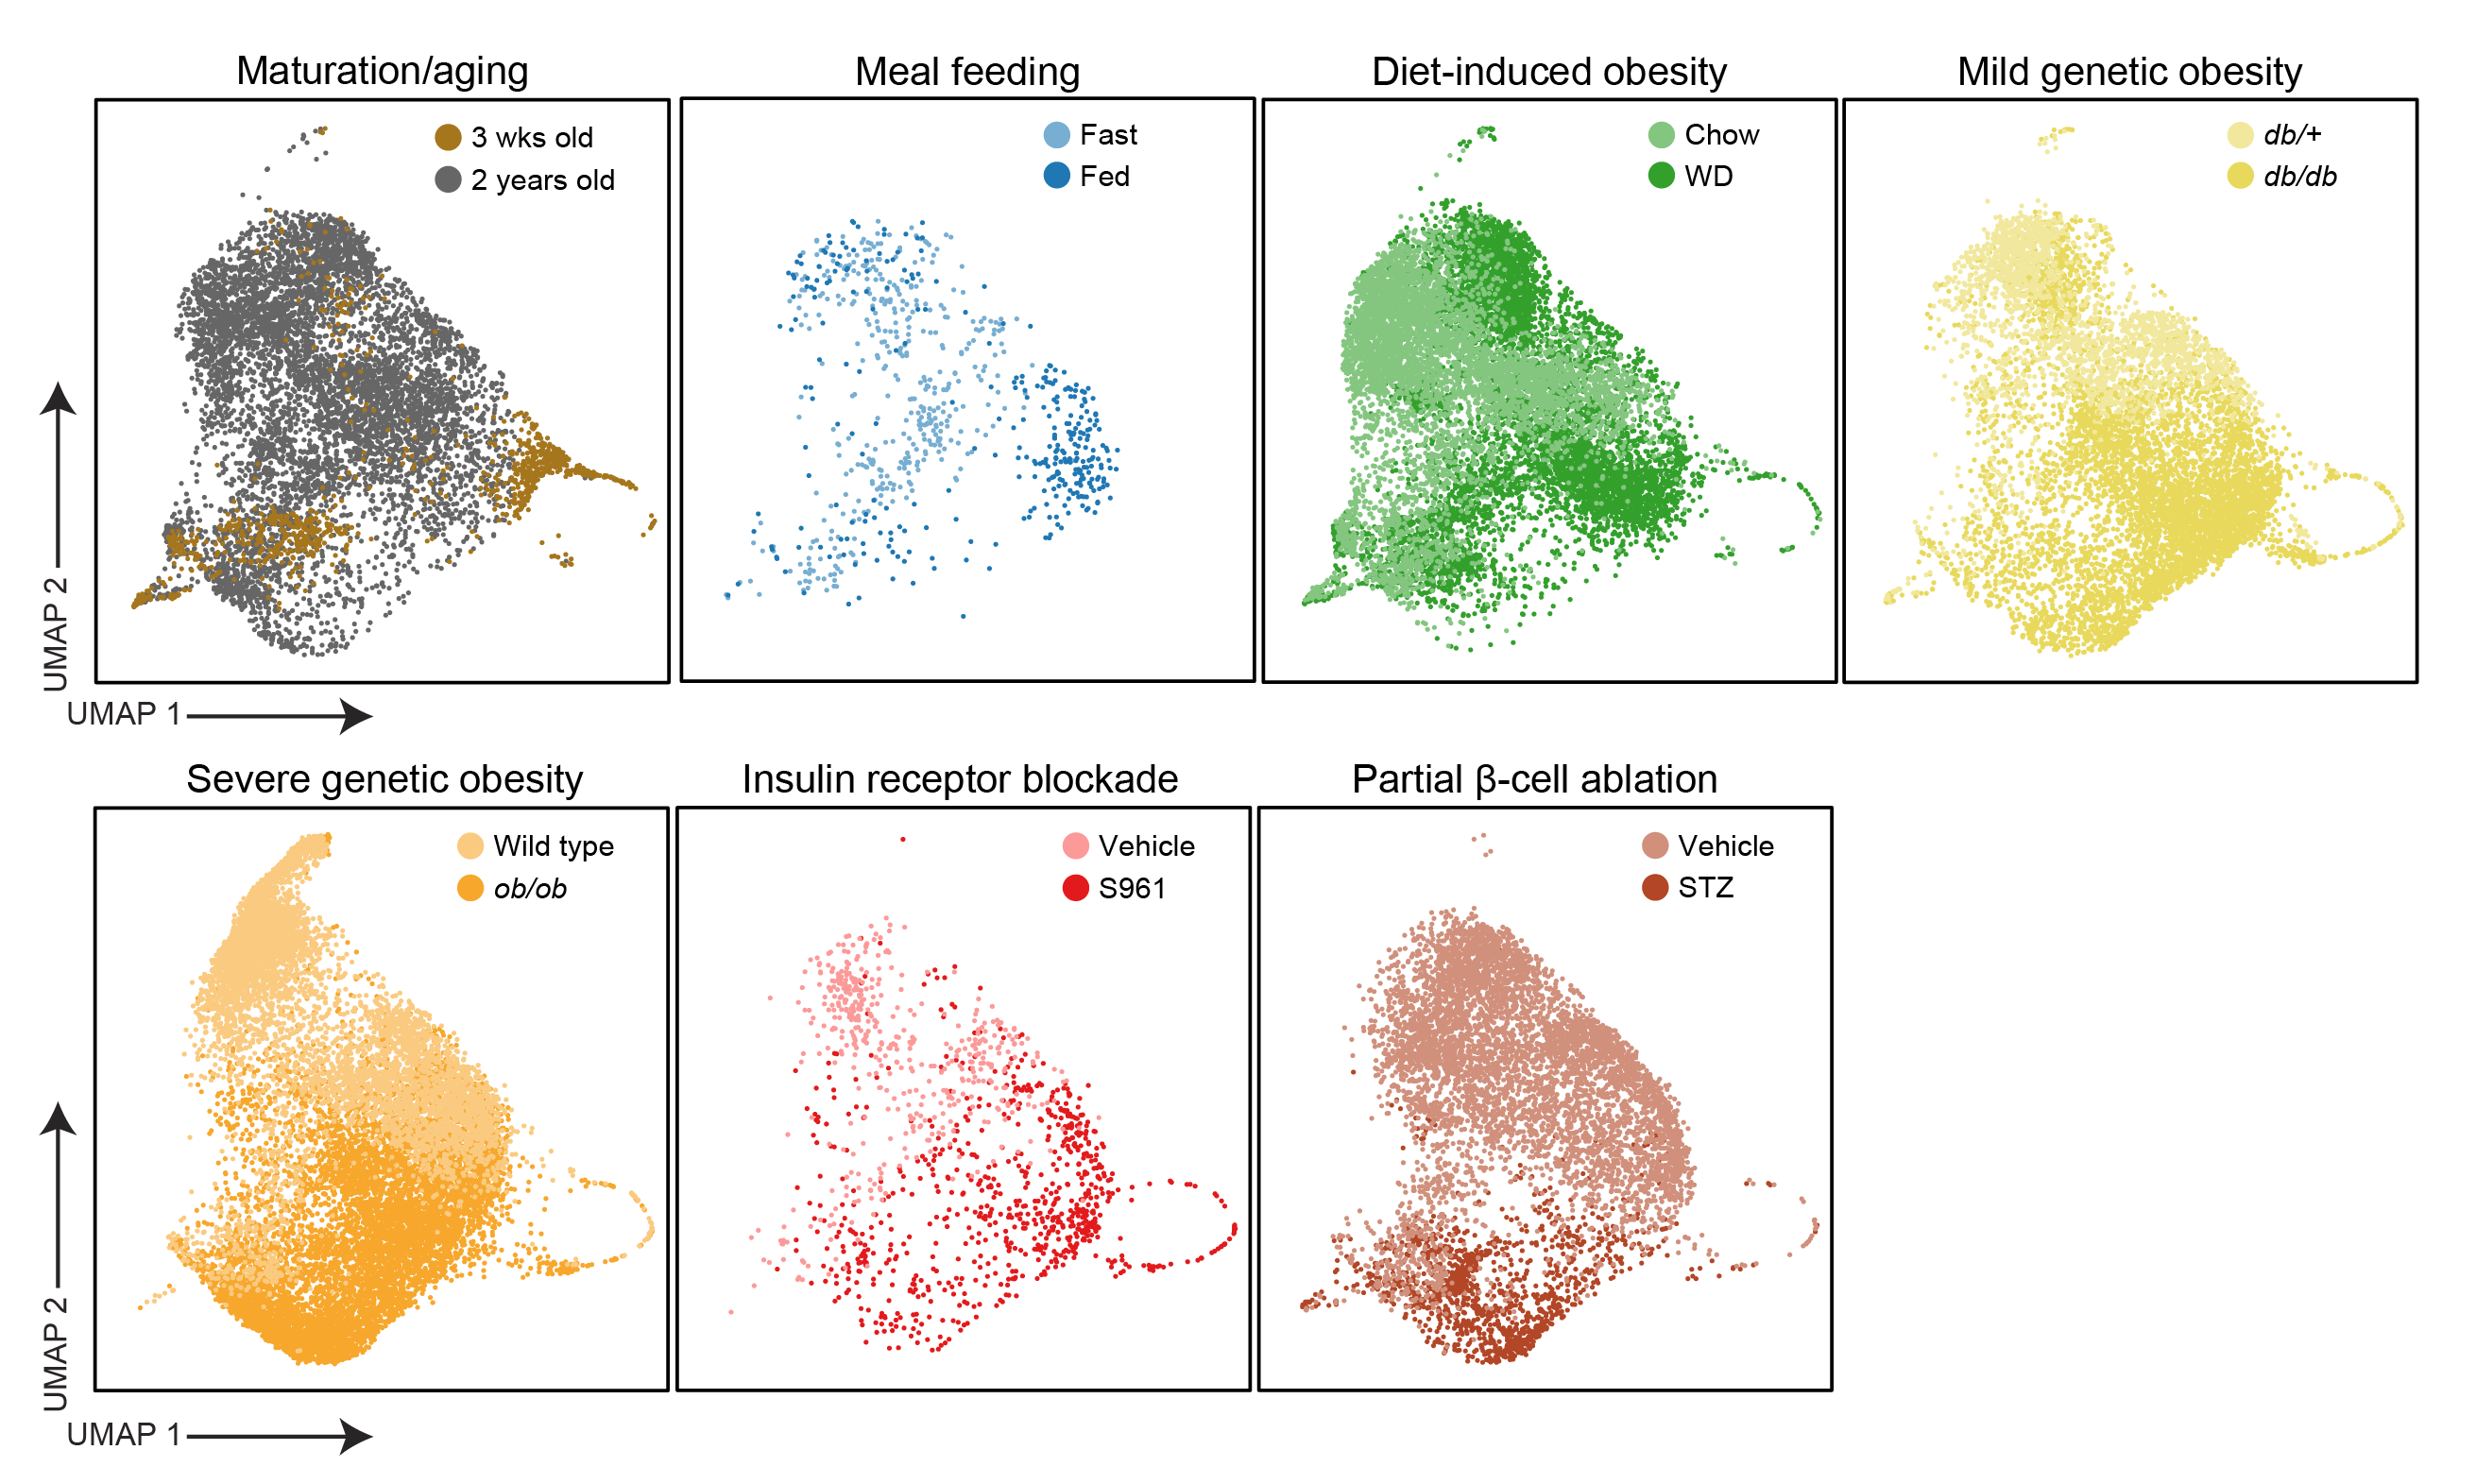
\includegraphics[width=\linewidth]{Appendix2/Fig/F3-4-01.png}
\caption[β-cell subset across seven studies]{}
\label{suppl_fig:chp3_betastudy}
\end{figure}

% \begin{figure}[H]
% \centering
% 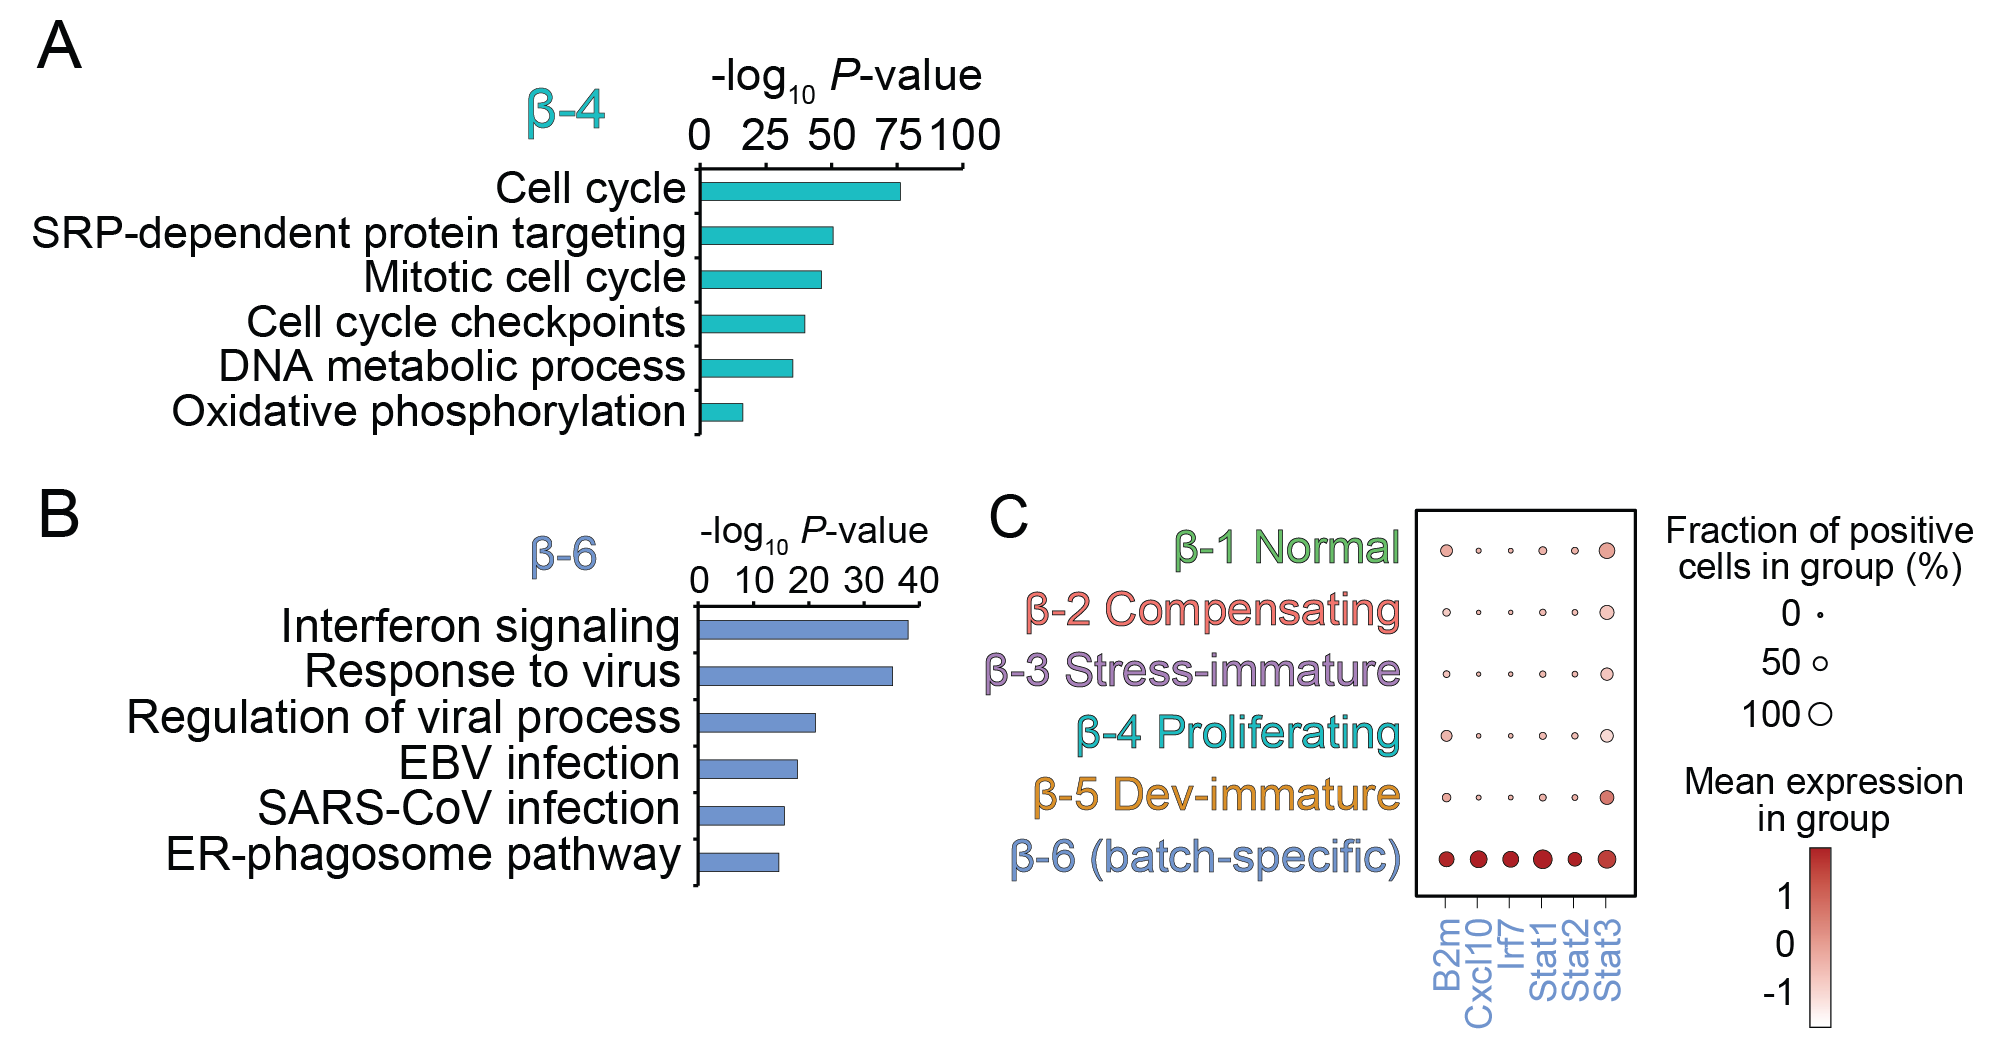
\includegraphics[width=\linewidth]{Appendix2/Fig/F3-1-v2-01.png}
% \caption[Characterization of β-cell subsets using enriched markers and gene ontology]{}
% \label{suppl_fig:chp3_betasubsets}
% \end{figure}


\begin{figure}[H]
\centering
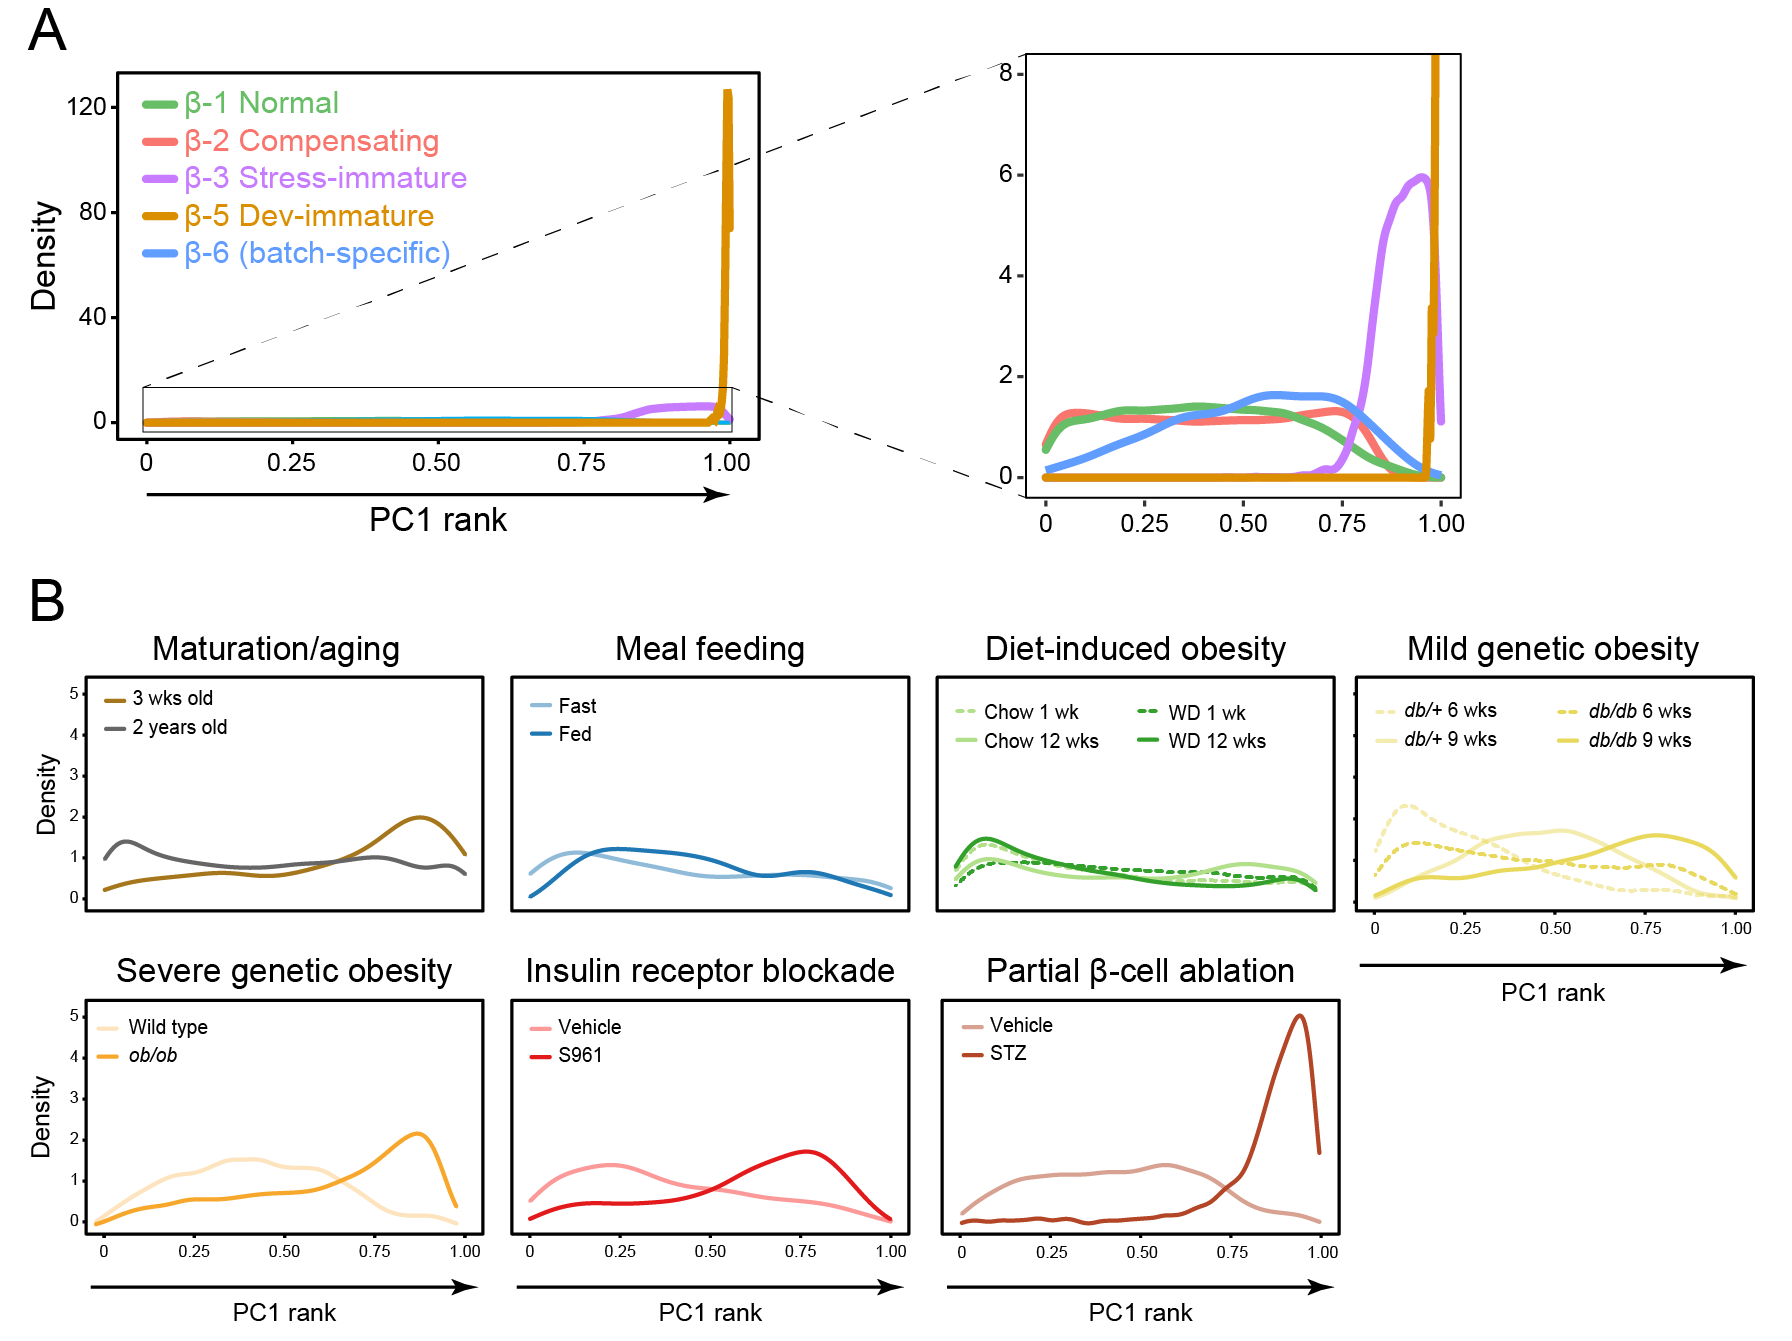
\includegraphics[width=\linewidth]{Appendix2/Fig/F3-7-02.png}
\caption[Loss of β-cell maturity across studies along PC1]{}
\label{suppl_fig:chp3_pc1}
\end{figure}


\begin{figure}[H]
\centering
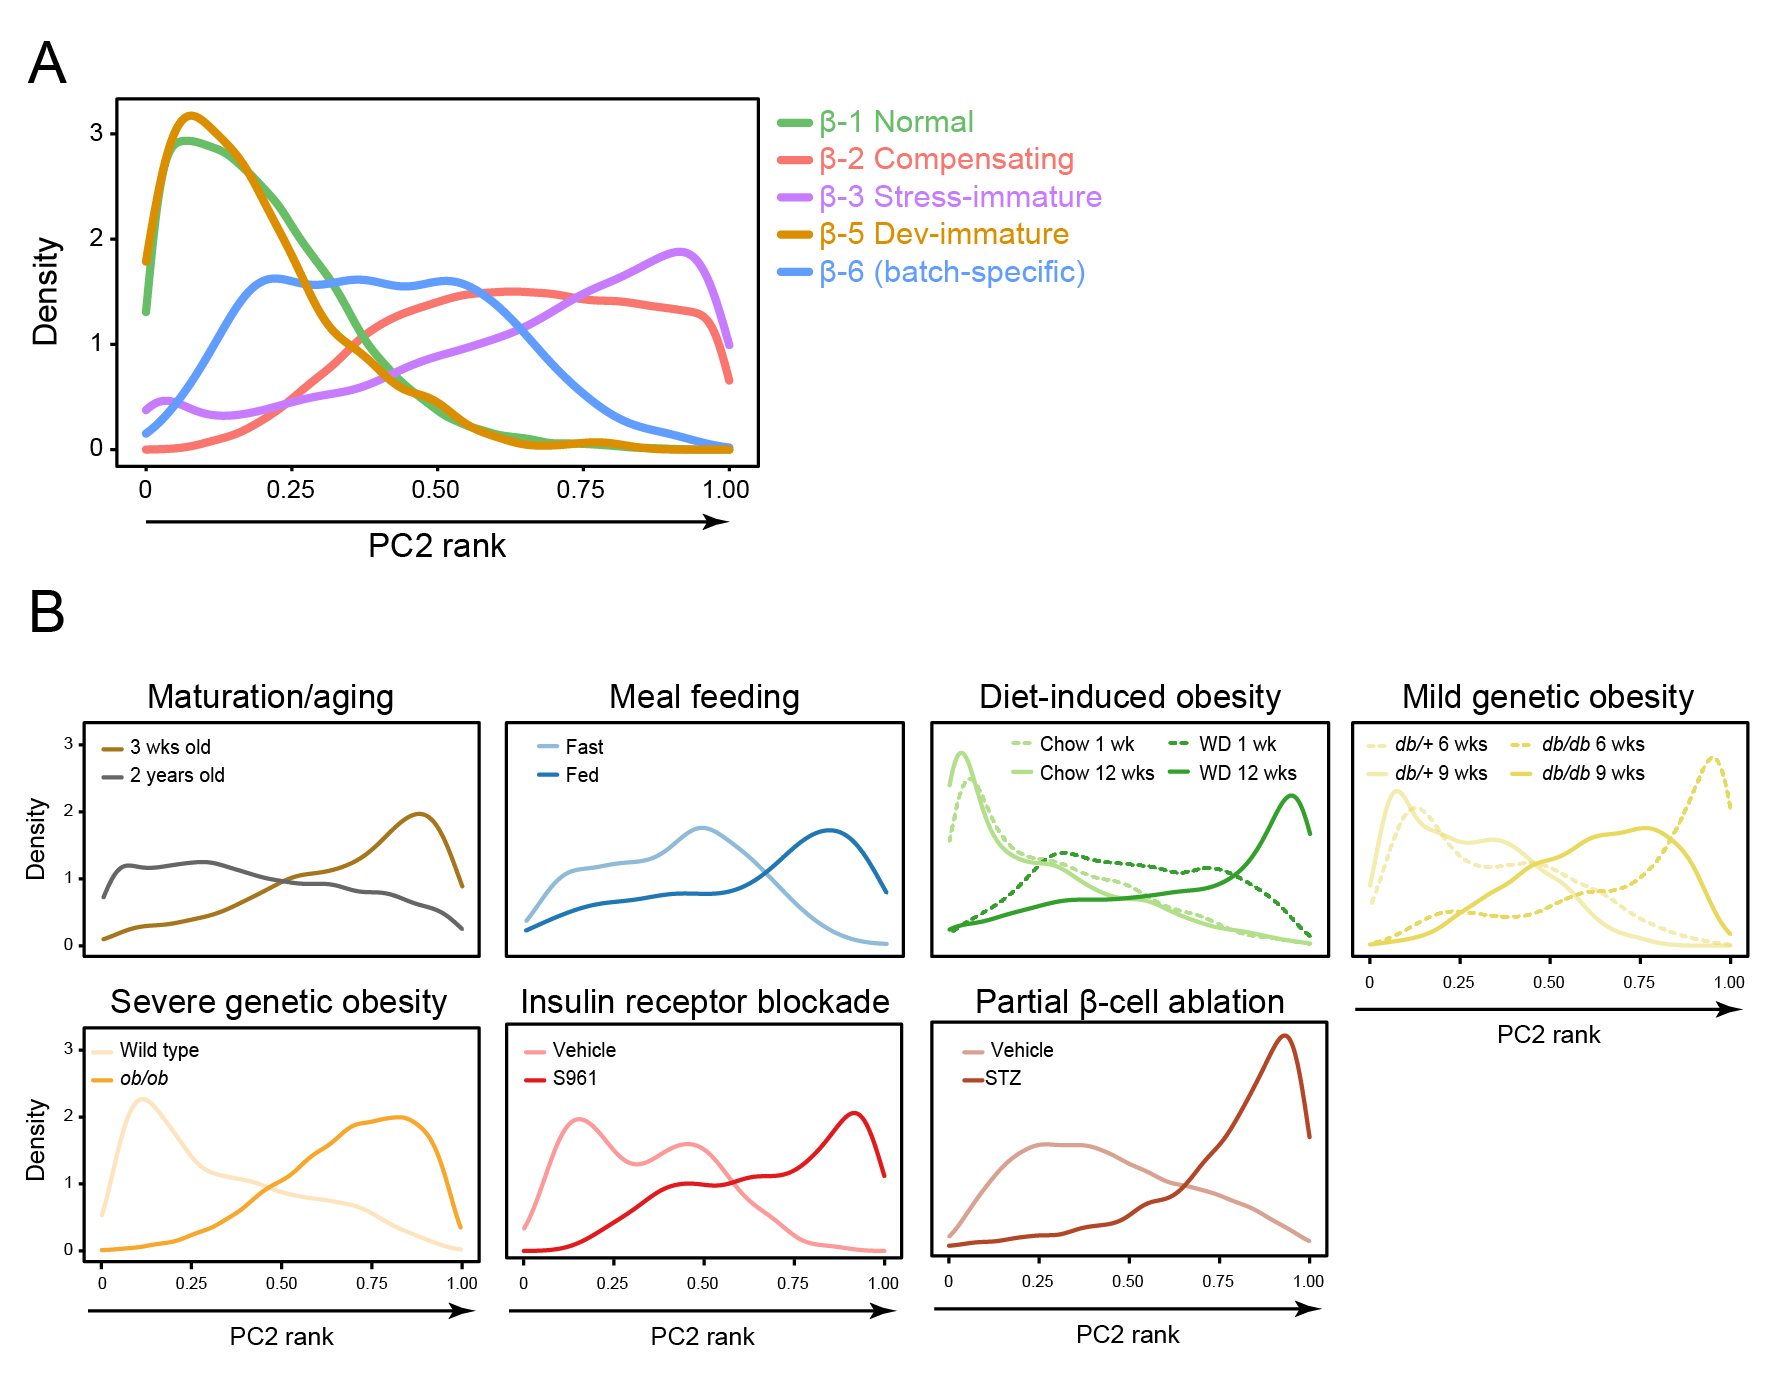
\includegraphics[width=\linewidth]{Appendix2/Fig/F3-7-03.png}
\caption[Increased β-cell workload across studies along PC2]{}
\label{suppl_fig:chp3_pc2}
\end{figure}

\begin{figure}[H]
\centering
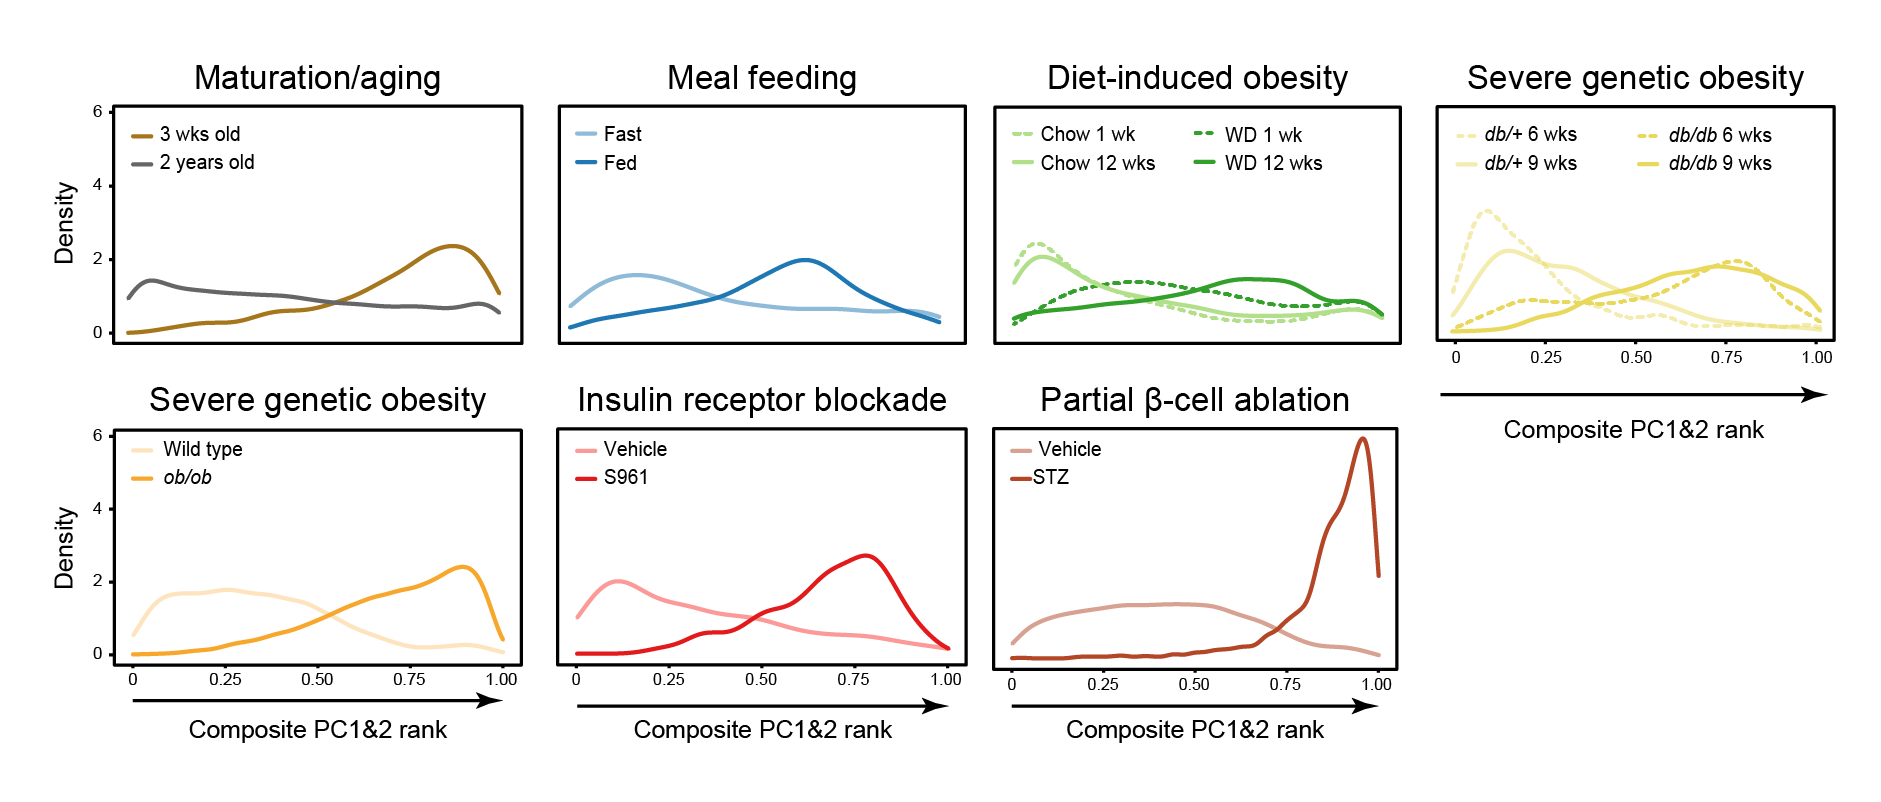
\includegraphics[width=\linewidth]{Appendix2/Fig/F3-7-01.png}
\caption[β-cell failure across studies along composite PC1 and PC2]{}
\label{suppl_fig:chp3_pc2}
\end{figure}

\begin{figure}[H]
\centering
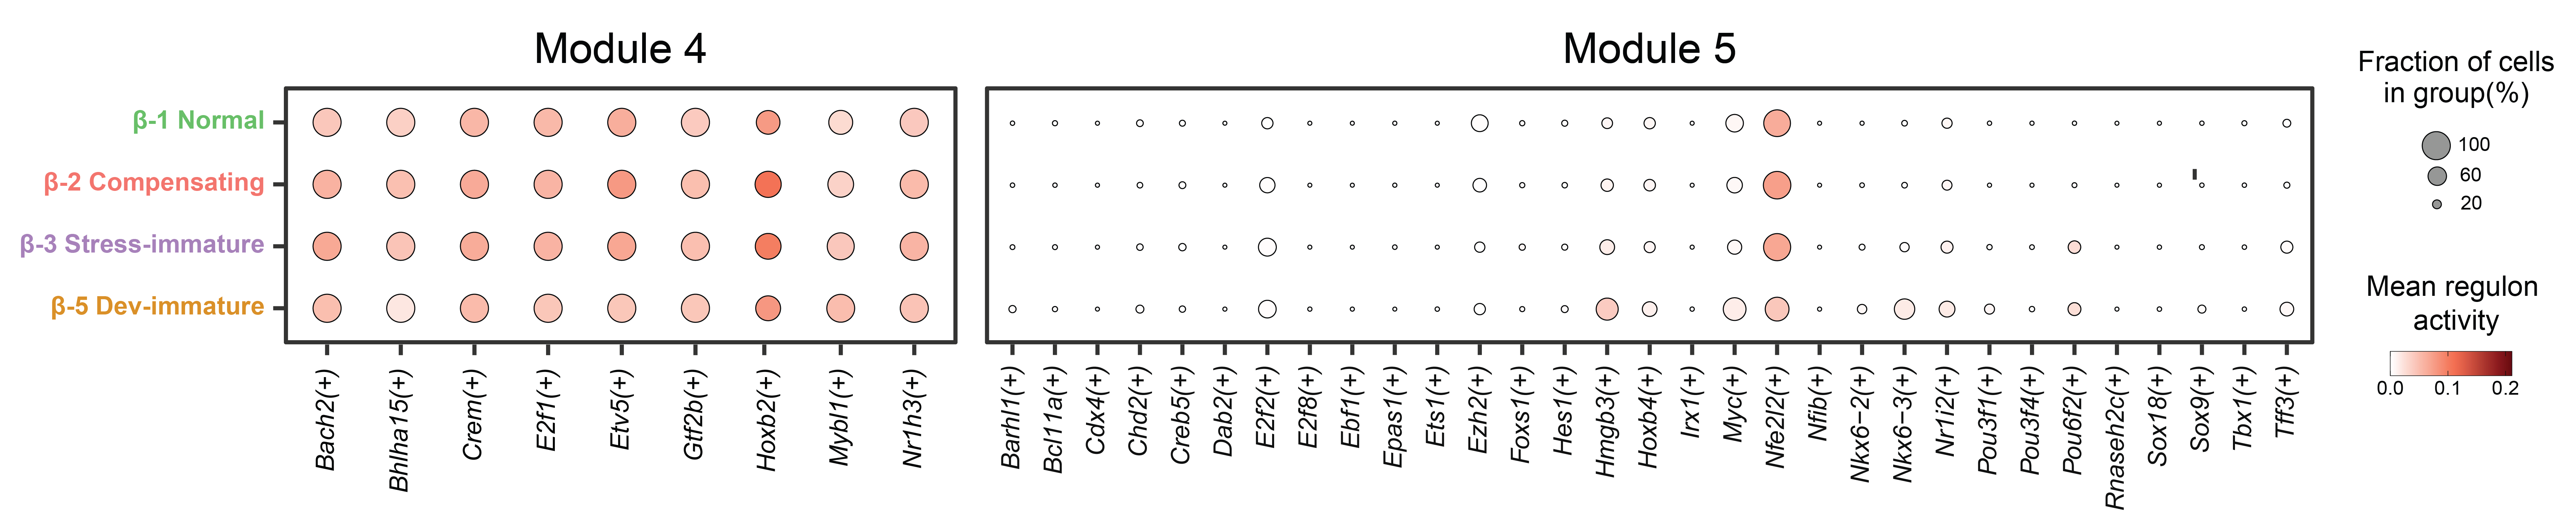
\includegraphics[width=\linewidth]{Appendix2/Fig/F3-12-04.png}
\caption[Mean regulon activity of all regulons in Module-4 and Module-5 of β-cell GRN]{}
\label{suppl_fig:chp3_GRNmods45}
\end{figure}

% \mysidecaption{0.4}{%
% \captionof{figure}[Gene-set scores in Aging/maturation study]{\textbf{Scores of five gene-sets in Aging/maturation study}}%
% }
% {%
% 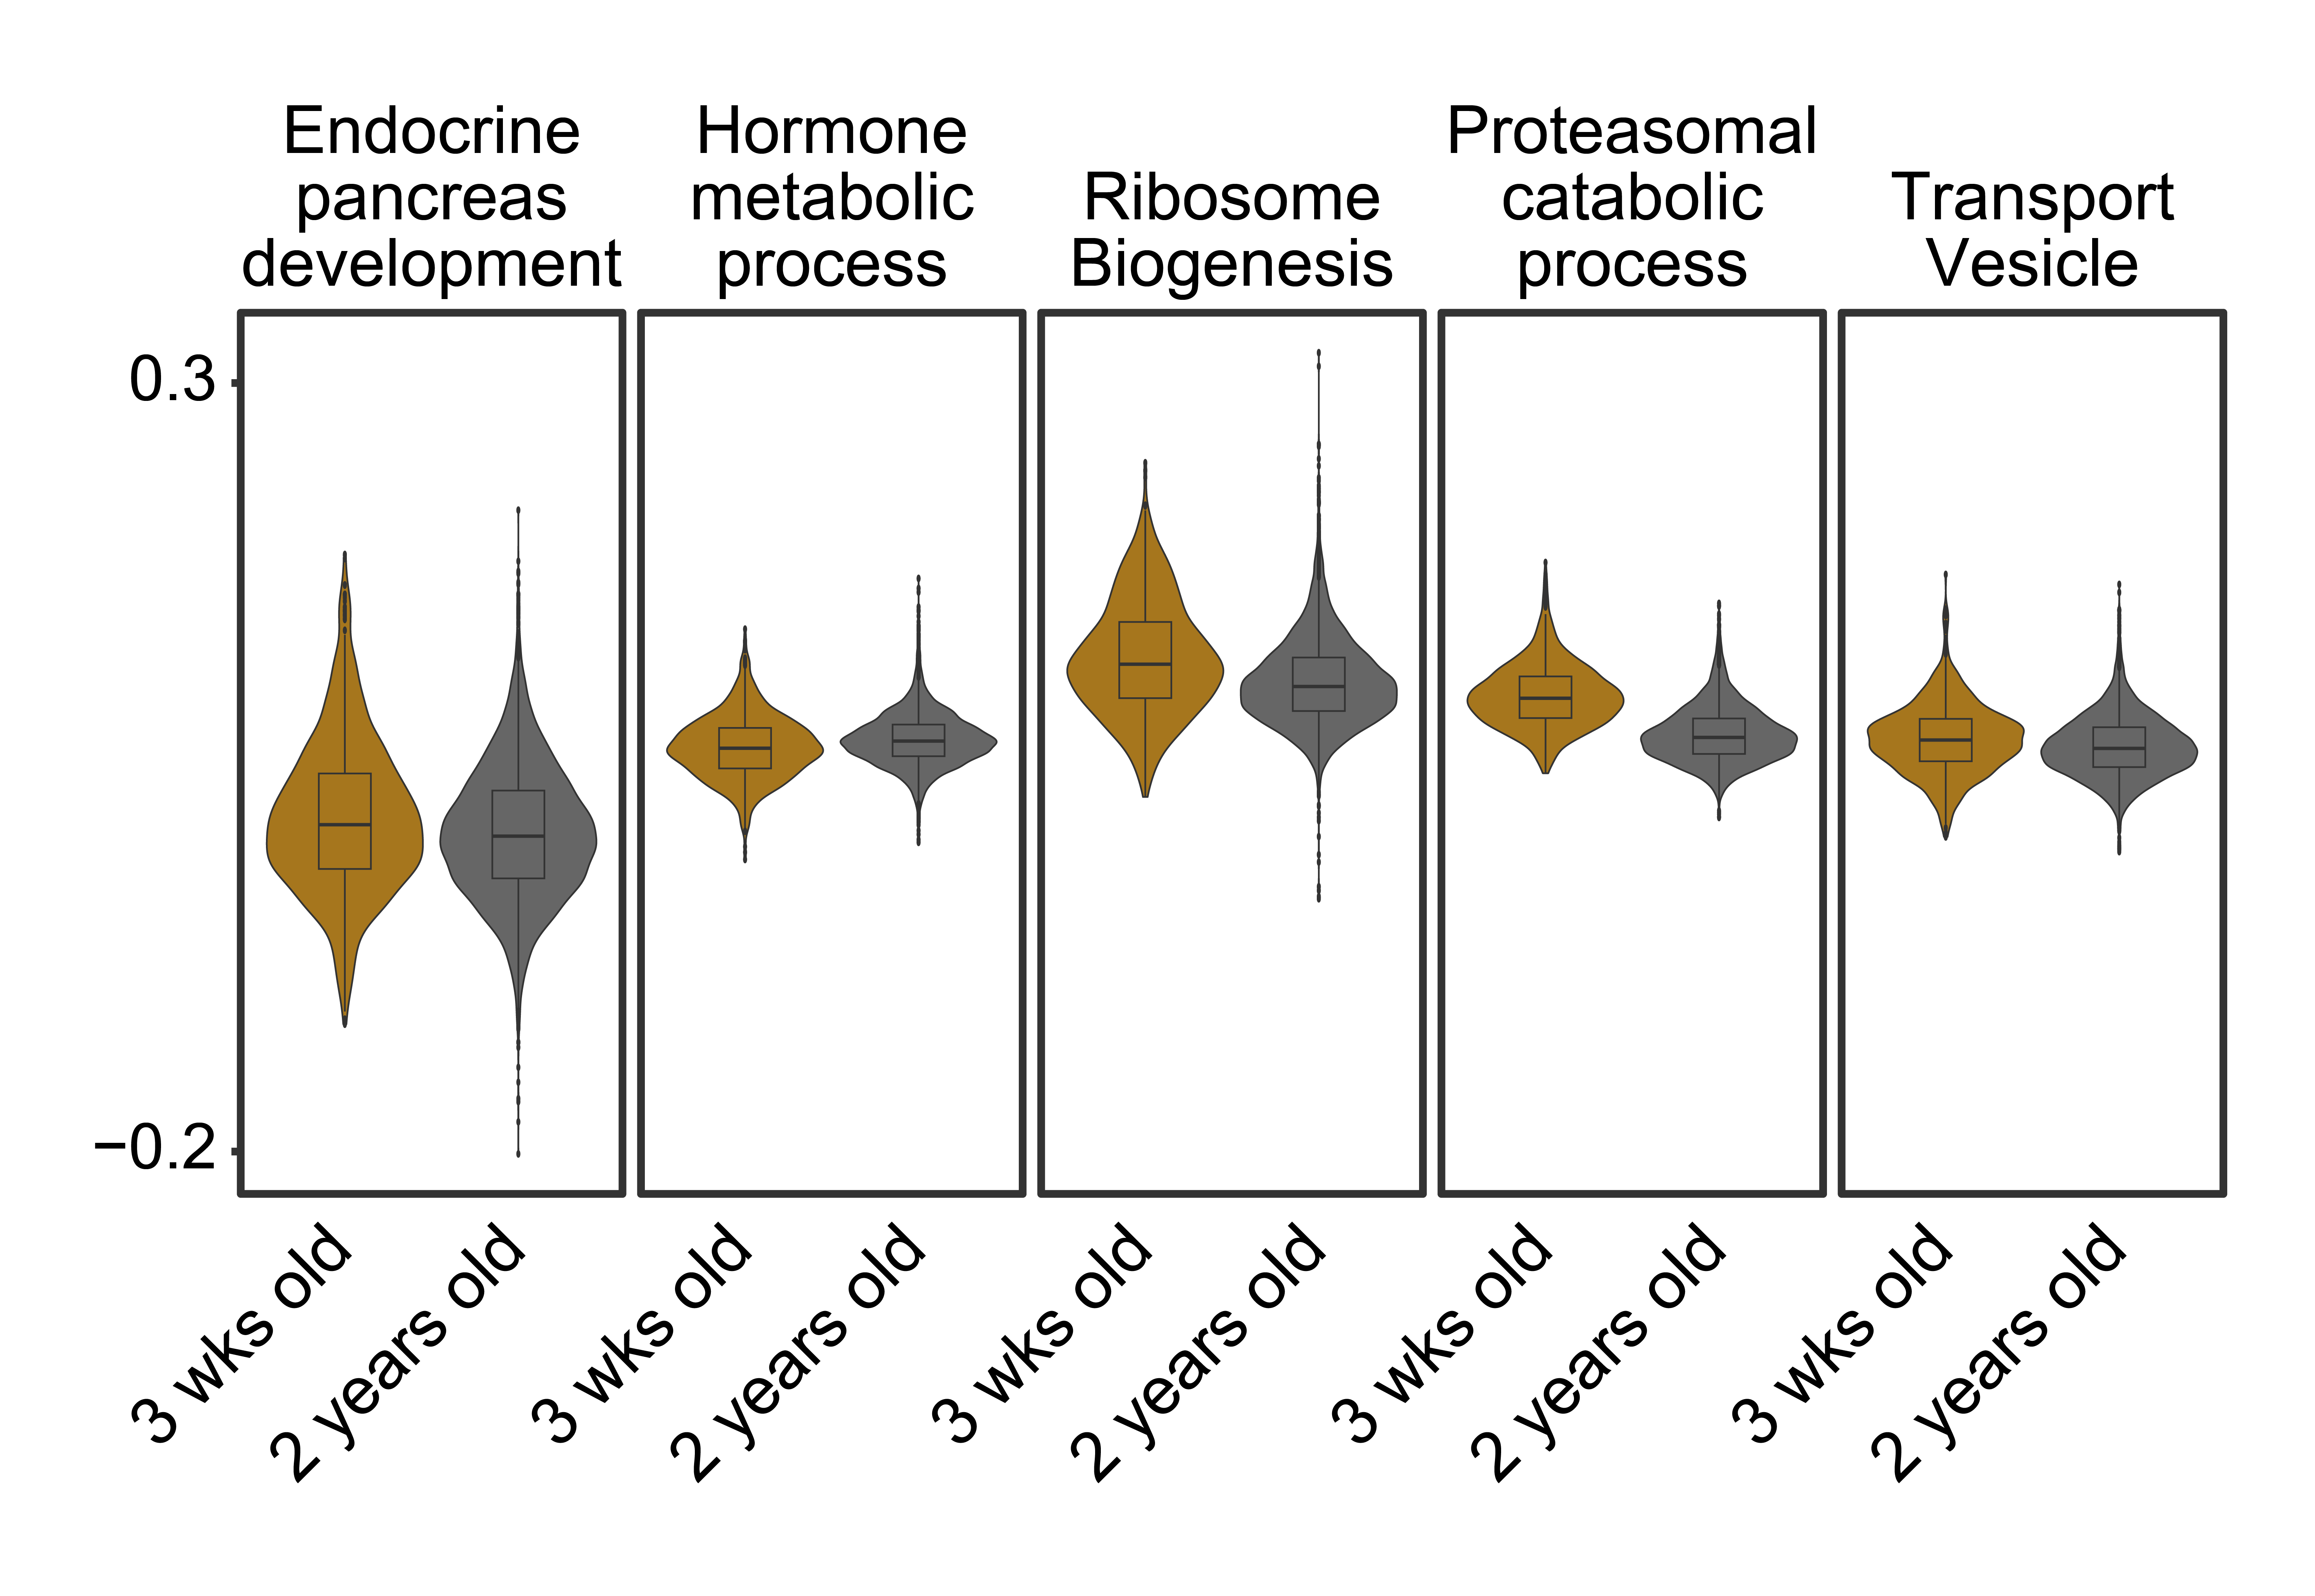
\includegraphics[width=9.5cm]{Appendix2/Fig/F3-14-01.png}%
% }[t]%

\begin{figure}[t]
\centering
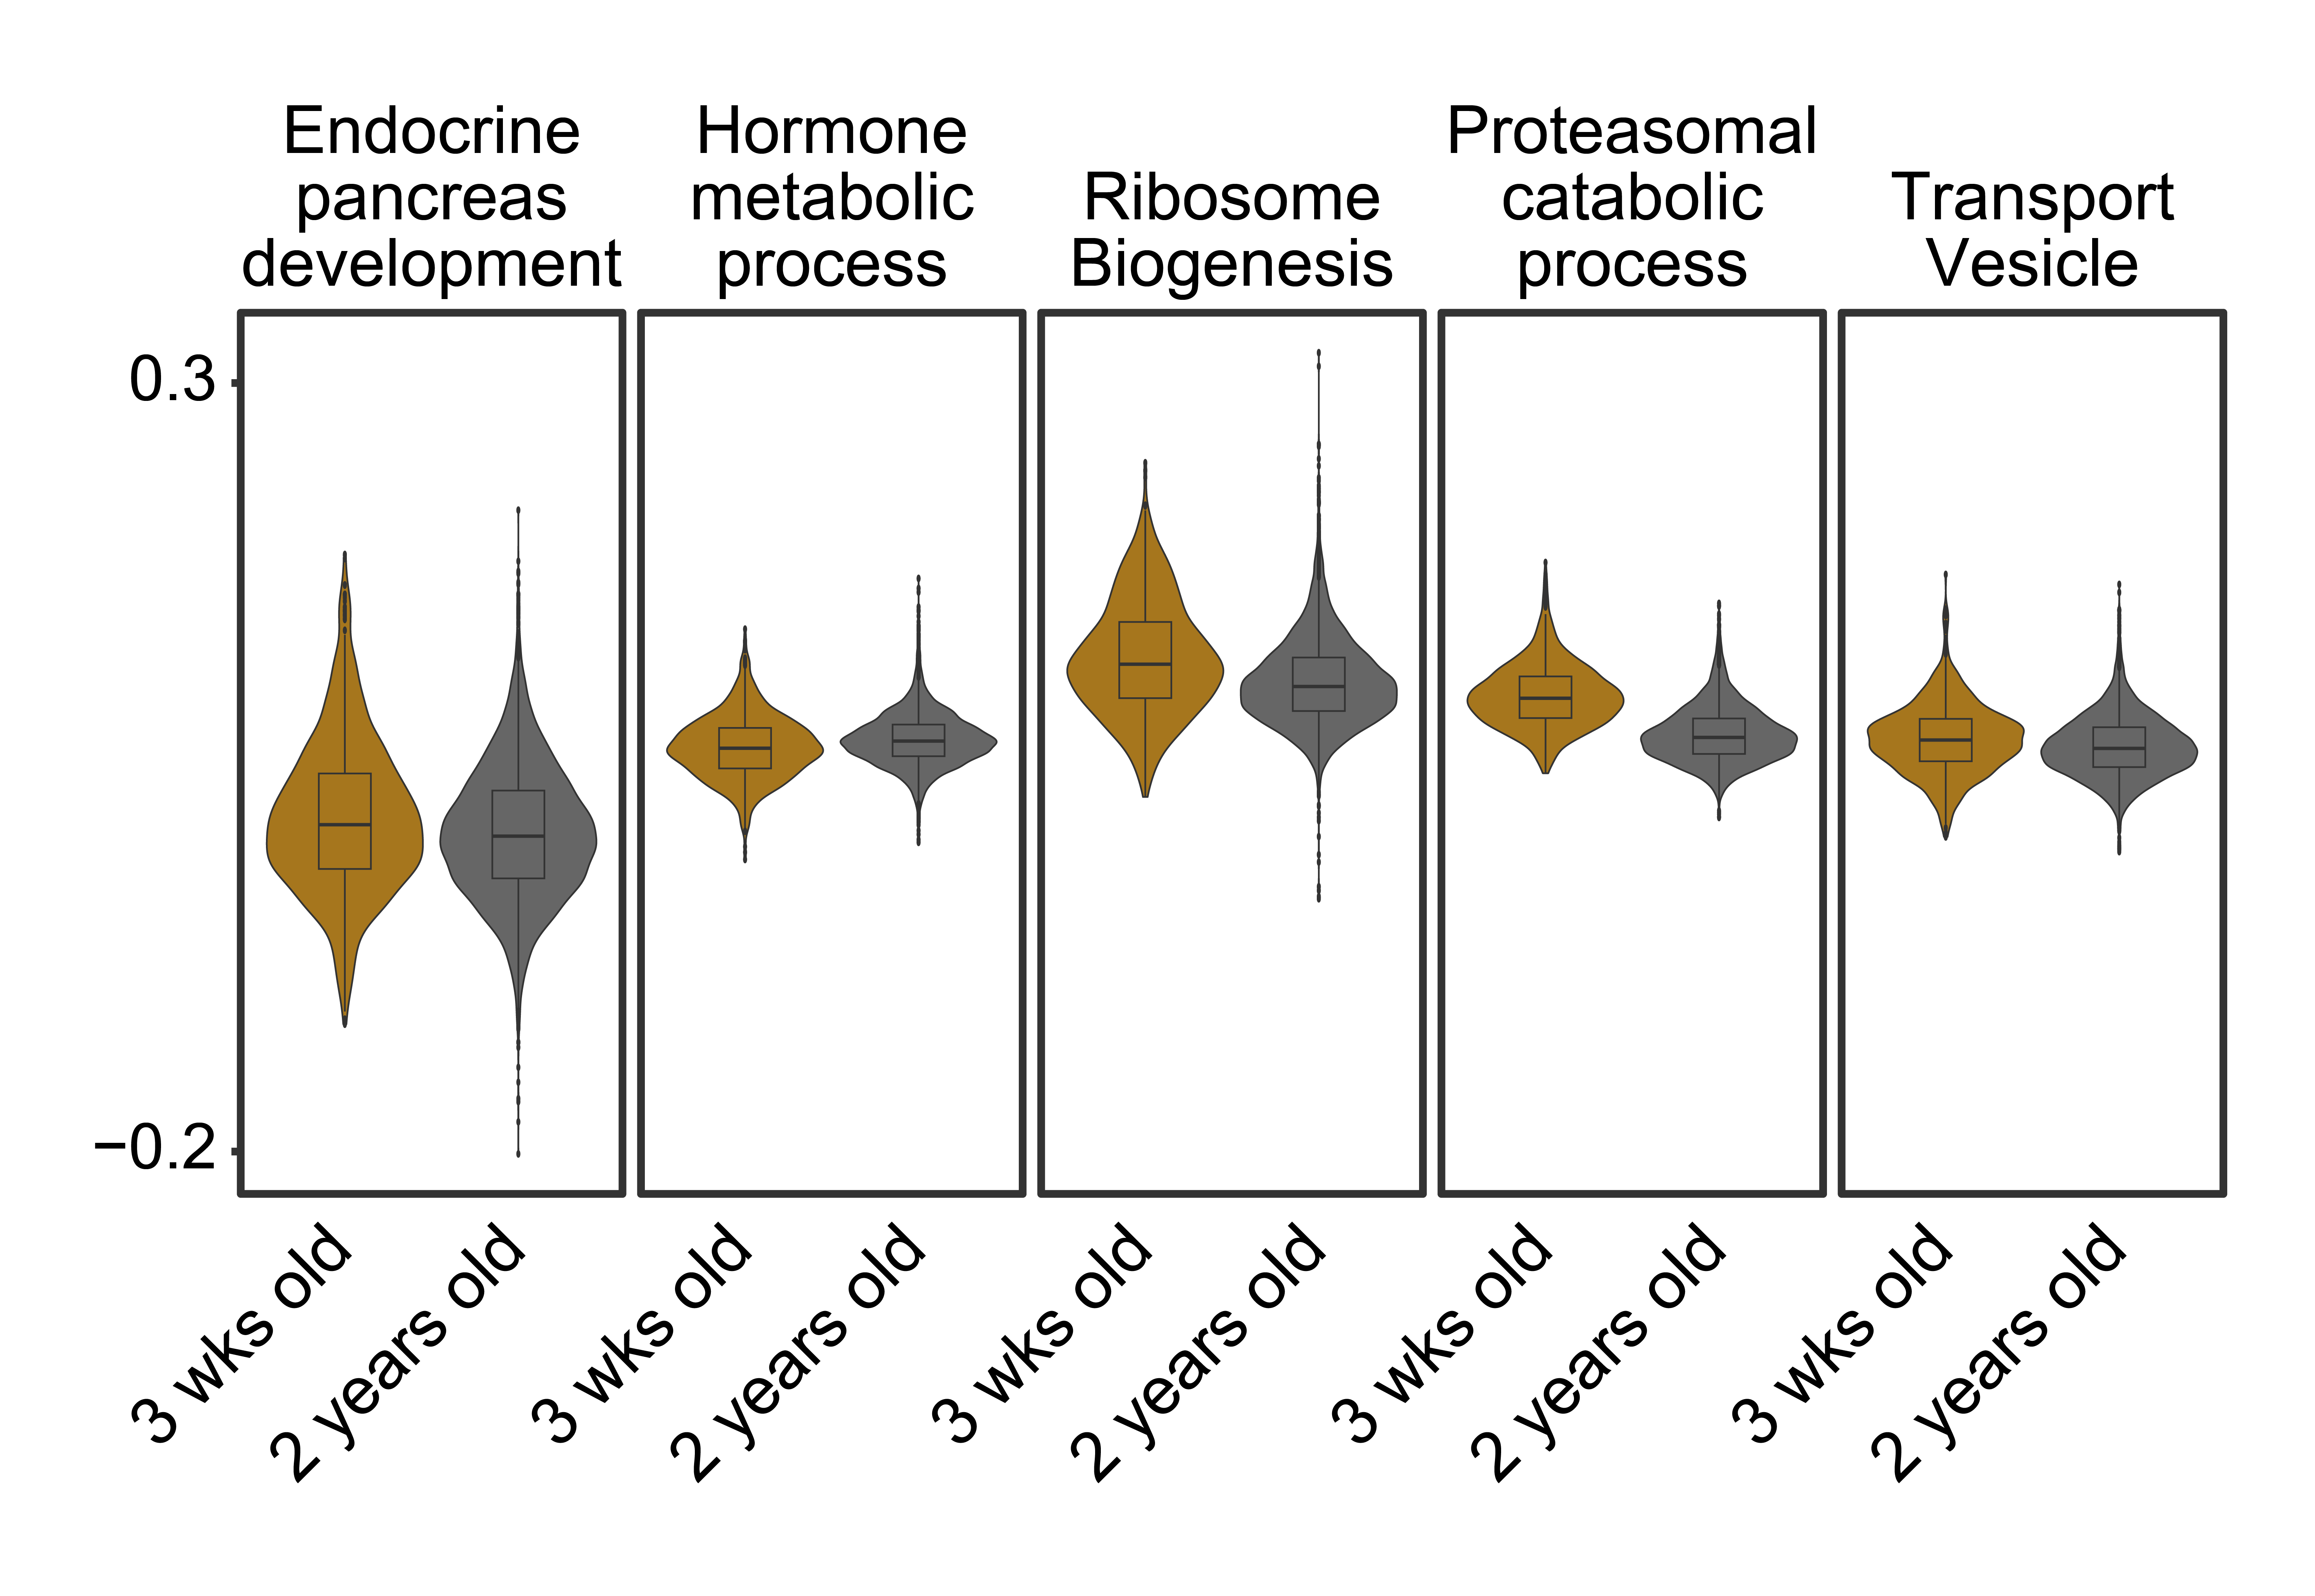
\includegraphics[width=11cm]{Appendix2/Fig/F3-14-01.png}
\caption[]{Gene-set scores in Aging/maturation study}
\label{suppl_fig:chp3_agingscores}
\end{figure}




% \begin{landscape}
\begin{figure}[H]
\centering
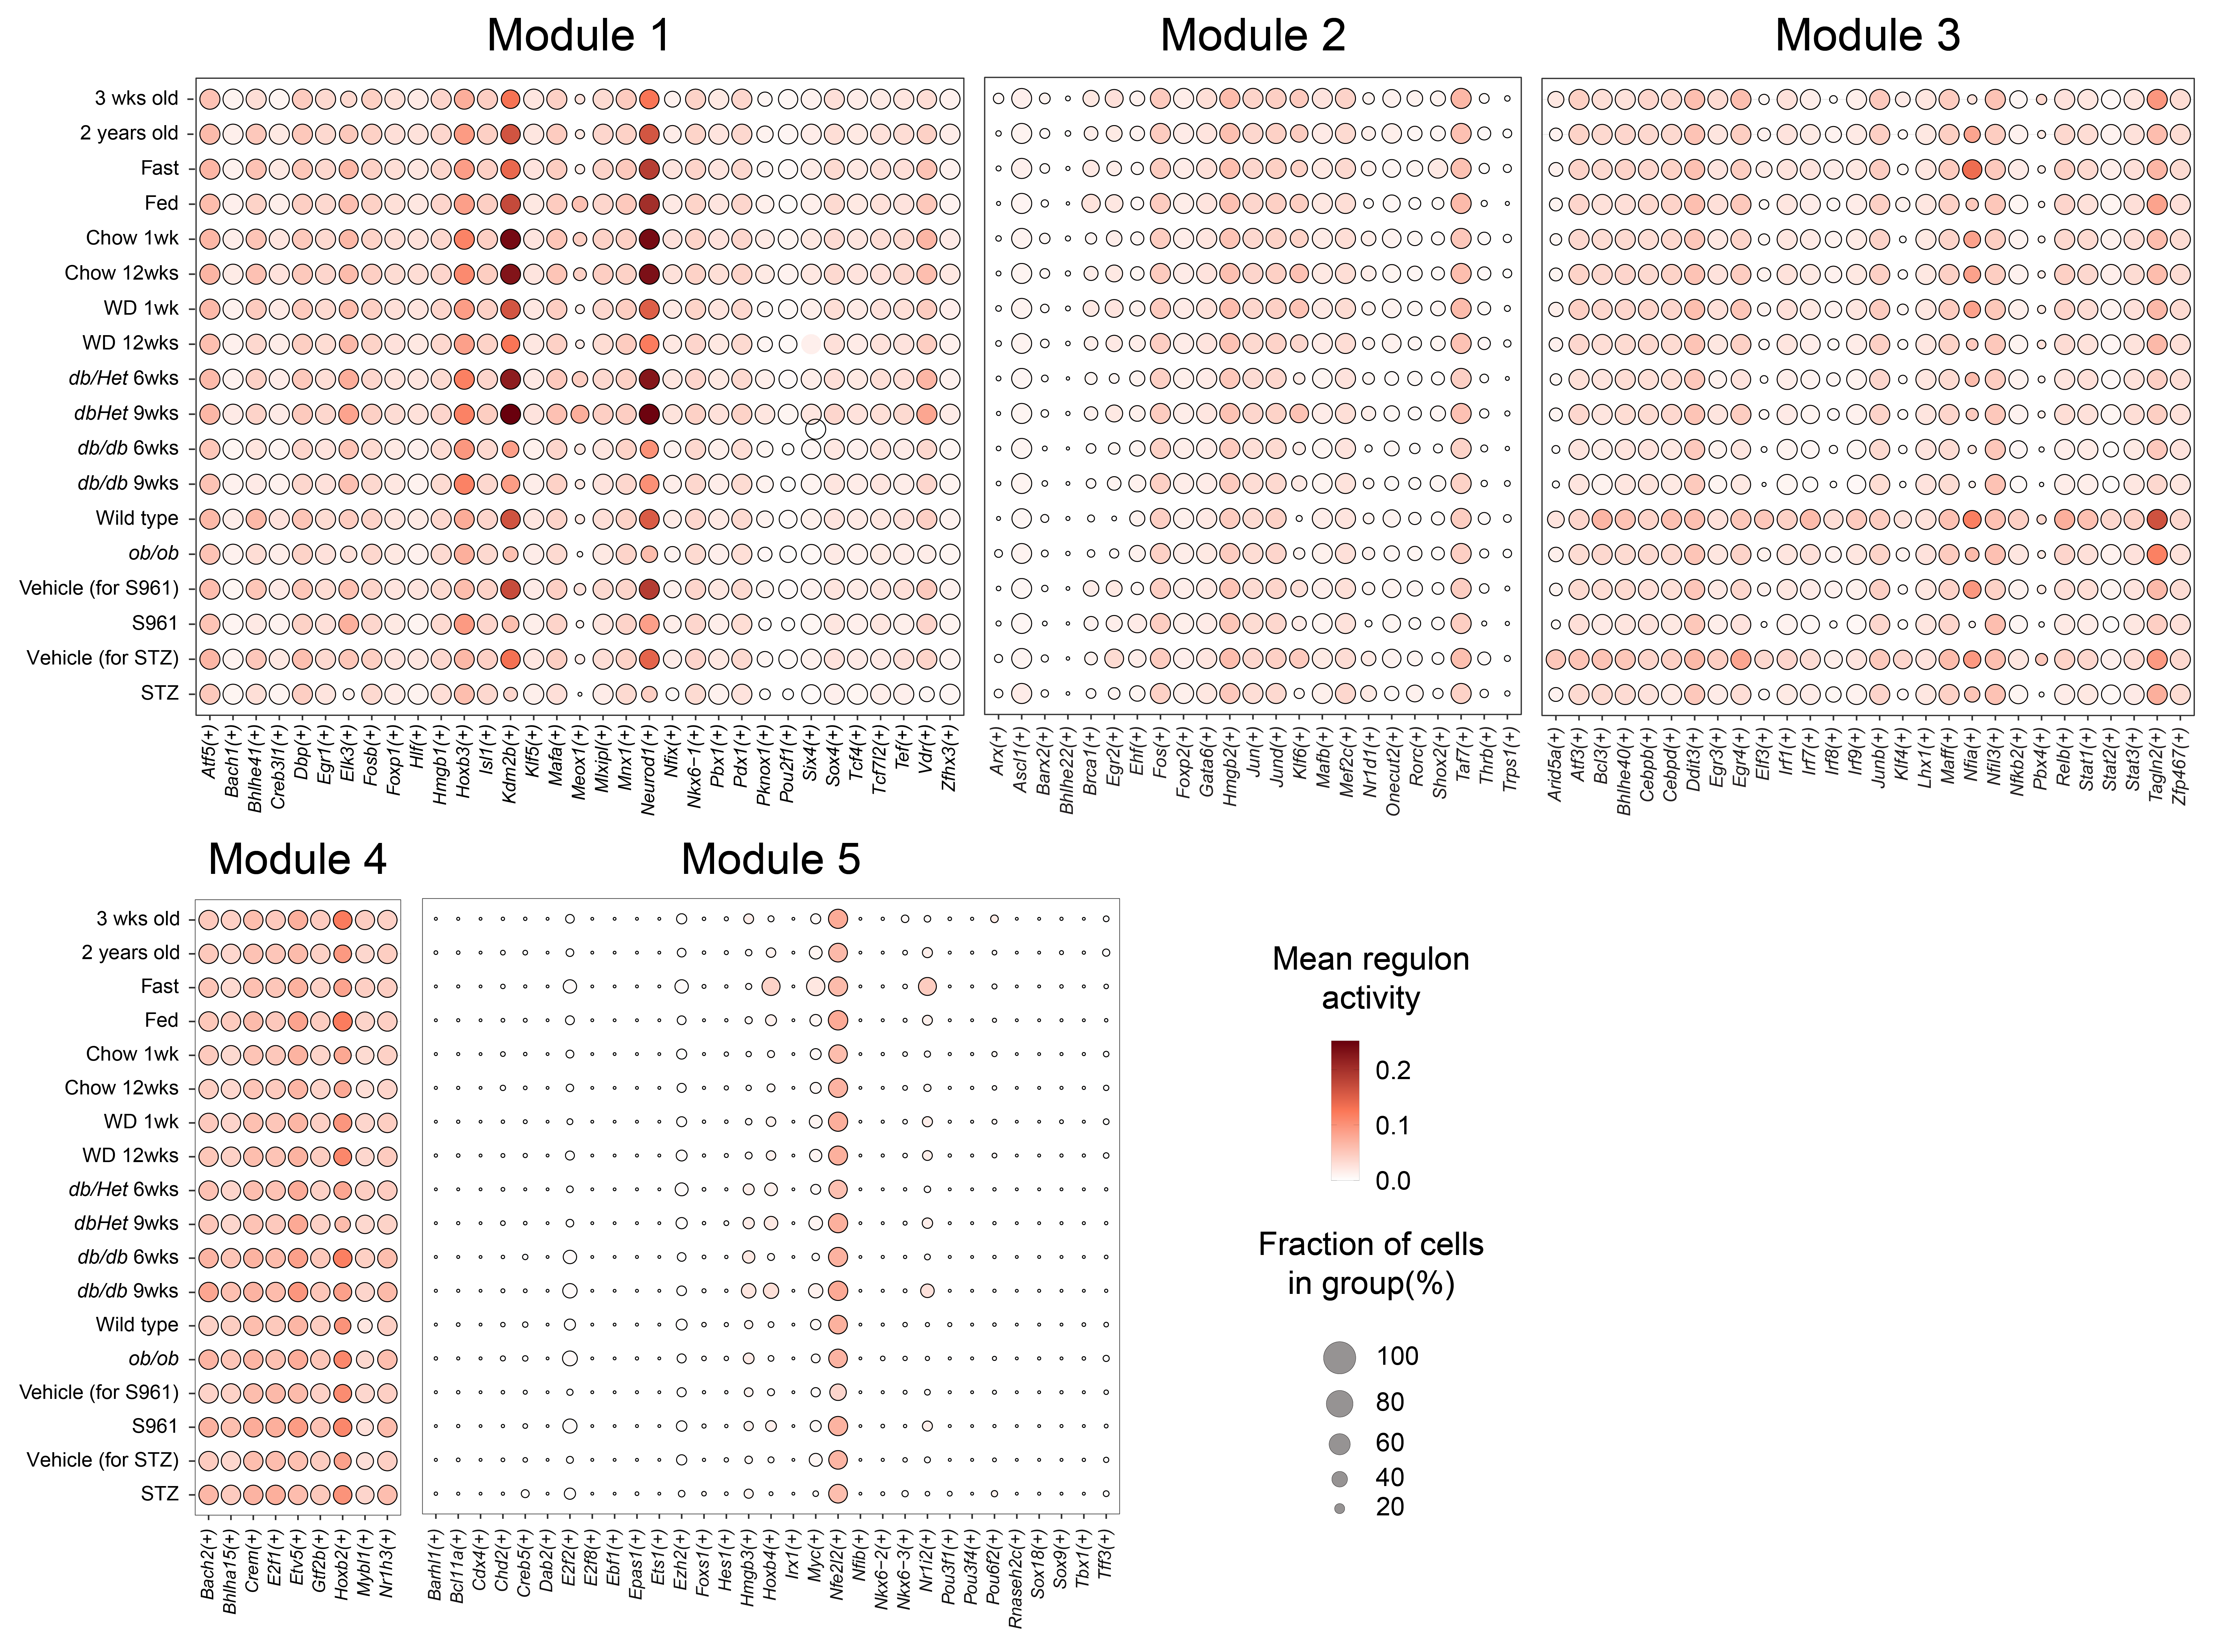
\includegraphics[width=\linewidth]{Appendix2/Fig/F3-15-01.png}
\caption{Intensity measure correlation}
\label{fig:IMs matrix correlation}
\end{figure}
% \end{landscape}